\documentclass[../Main.tex]{subfiles}

\begin{document}
\chapter{Statistical Machine Learning}

\intro{

}

\section{Basics}
\begin{figure}[H]
    \centering
    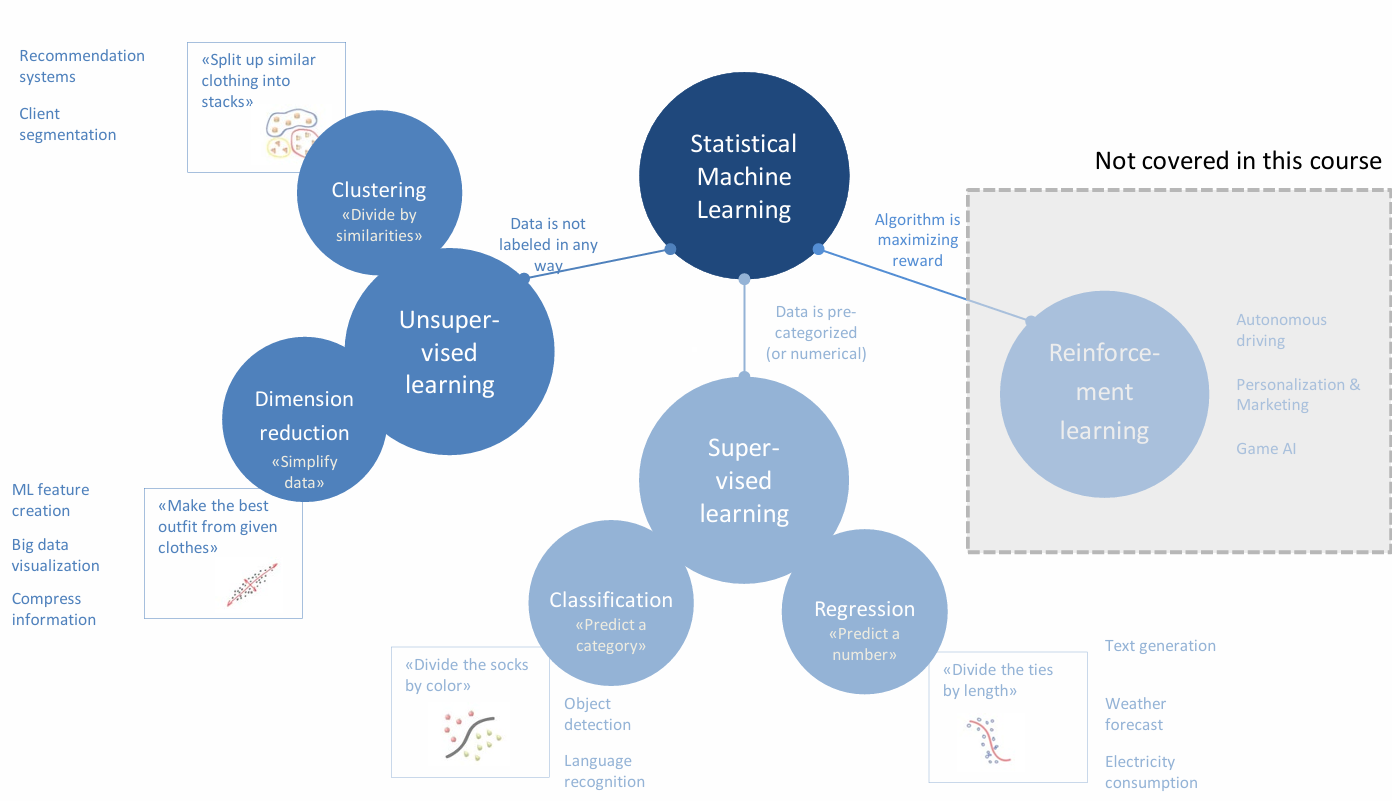
\includegraphics[width=1\linewidth]{Images/overview.png}
    \caption{Overview}
\end{figure}

\defn{Correlation and Causation}{
    \textbf{REMEMBER!} Correlation does not imply causality!
}

\defn{No Free Lunch}{
There is not one method which will 
beat all the other methods all the 
time. The better the assumptions of the 
method match the true state of nature, 
the better a particular method performs. This is sometimes referred to as the 
"No Free Lunch Theorem".
}

In StatML we want to create mathematical models based on data.
We assume a fixed but unknown relationship between the input variables \(X\) (predictors) and our
output (dependent variable) \(Y\).

Given a dataset (usually represented by a input vector \(X\)):
\begin{equation*}
    X = (X_1, X_2, \dots, X_p)
\end{equation*}
Find a function that as good as possible models our unknown relationship:
\begin{equation*}
    Y = f(X) + \varepsilon
\end{equation*}
One of the main goals is to minimize the reducible error \(\varepsilon\). See subsection "Error" for more.

\defn{Inference vs Prediction}{
    \begin{itemize}
        \item In \textbf{inference} we are interested in understanding the relationship between predictors and response.
        \item The goal of \textbf{prediction} is to calculate new values \(\hat{y}\) with given predictors \(X_i\).
    \end{itemize}
}

When choosing a method or model. There is a \textbf{clear tradeoff between flexibility and model interpretability}.
One can say that a model which is easier to interprete, is in turn also less capable to predict accurate values, in comparison
to models which are less interpretable.

\begin{figure}[H]
    \centering
    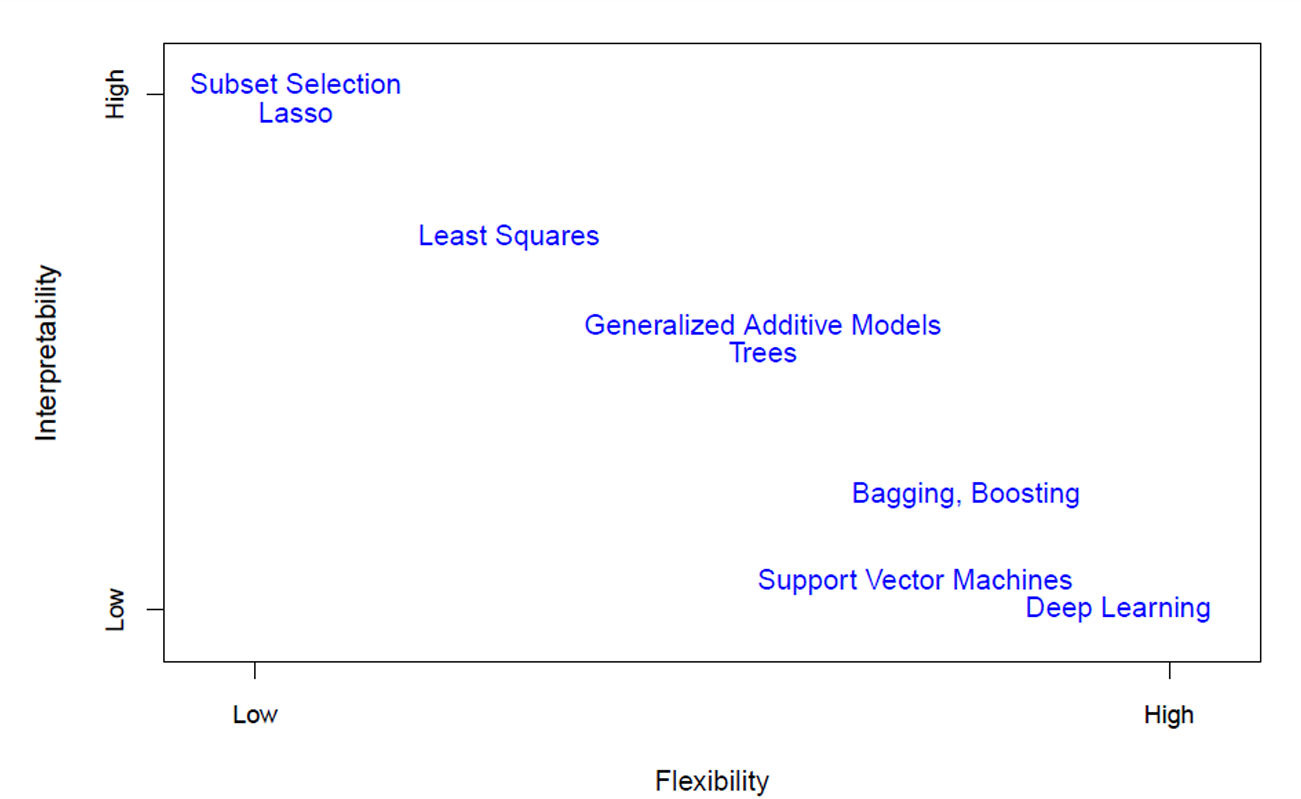
\includegraphics[width=0.75\linewidth]{Images/model-interpretability.png}
    \caption{Model Interpretability Tradeoff}
\end{figure}

\defn{Estimation Aproaches}{
    \begin{description}
        \item[Parametric] Assumptions are made about the functional form of \(f(X)\), where some missing parameters need to be learned. For example a simple linear model assumes form: \(f(X)=\beta_0+\beta_1X_1\).  If the form of \(\hat{f}(X)\) is far from \(f(X)\), then this approach achieves badly.
        \item[Non-Parametric]  Methods that make no assumptions about the functional form of \(f(X)\).
    \end{description}
}

We define two big method subcategories of statistical machine learning methods.
\defn{Supervised Learning vs Unsupervised}{
    \begin{description}
        \item[Supervised] For each input vector \(X\), its corresponding dependent variable \(Y\) is known.
        \item[Unsupervised] There is no corresponding dependent variable \(Y\) known. 
    \end{description}
}

\subsection{Error}
\defn{Error}{
    The Output (dependable variable) depends not only on the input, but also a from \(X\) 
    \textbf{indepentend zero mean error term} \(\epsilon\). Even a perfect prediction function \(f(x_i)\) has a 
    \textbf{irreducible error} \(\epsilon\).
    Error is introduced by internal as well as external factors:
    \begin{itemize}
        \item Random Measurement Error
        \item Systematic Errors e.g. humidity
    \end{itemize}

    If the estimated \(\hat{f}(X)\) is not equal to the true function, 
    there is the possibility to learn a better relationship between input and output, this is called \textbf{reducible error}. 
}

\exm{Error Terms with MSE}{
    One can show using algebra that the average error consists of two terms:
    \begin{equation}
        \begin{split}
            MSE&=E\{(Y-\hat{Y})^2\}\\
            &=(1)E\{(f(X)-\hat{f}(X))^2\}+(2)Var(\epsilon)\\
            (1)\text{Reducible Error }&+(2)\text{Irreducible Error}
        \end{split}
    \end{equation}
}

\newpage
\subsection{Bias-Variance}

\begin{figure}[H]
    \centering
    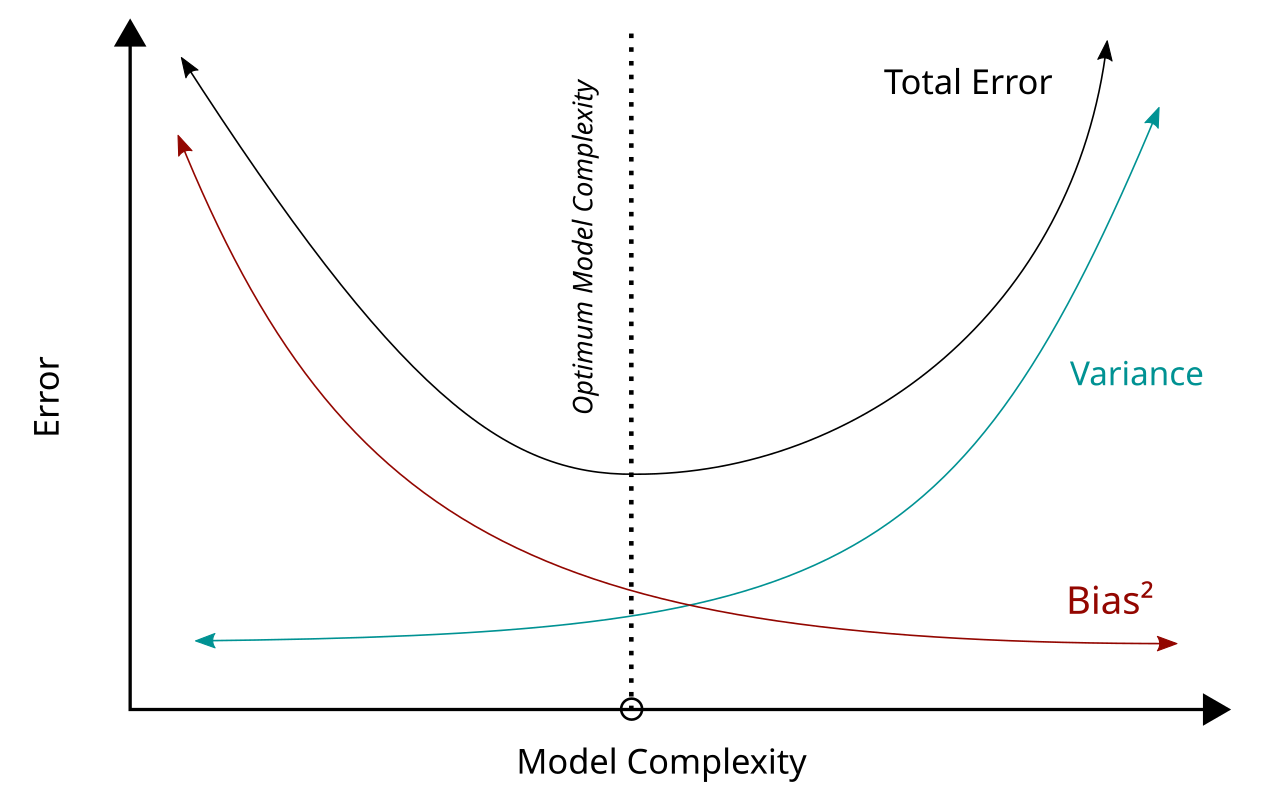
\includegraphics[width=0.5\linewidth]{Images/Bias_and_variance_contributing_to_total_error.svg.png}
    \caption{Bias Variance Tradeoff}
\end{figure}
The \textbf{expected test MSE} is the sum of a \textbf{variance} term, a \textbf{bias} term squared and the \textbf{irreducible error}.  Its defined as the average test MSE that would be obtained if \(f(X)\) is estimated repeatedly using a large number of training sets at tested at \(x_0\).
\begin{figure}[H]
    \centering
    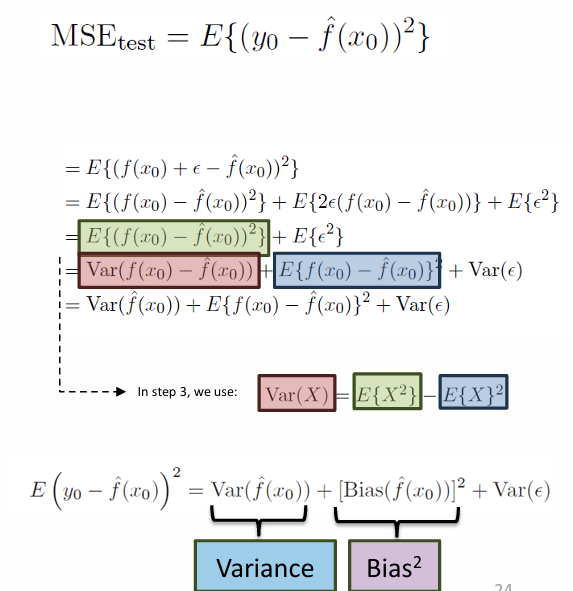
\includegraphics[width=0.5\linewidth]{Images/bias-variance-test-mse.png}
    \caption{Test MSE Equivalent}
\end{figure}

The \(\sqrt{variance}\) refers to the amount by which the estimate would change,
if we estimated using a different training set. 
Ideally the training set should have little influence on how the method estimates, this is typical for \textbf{low flexibility} methods.

The bias refers to the error introduced by approximation using a model that is \textbf{too simple} (low flexibility)
to capture the \textbf{true shape} of a function, this will result in \textbf{high bias}.

\begin{figure}[H]
    \centering
    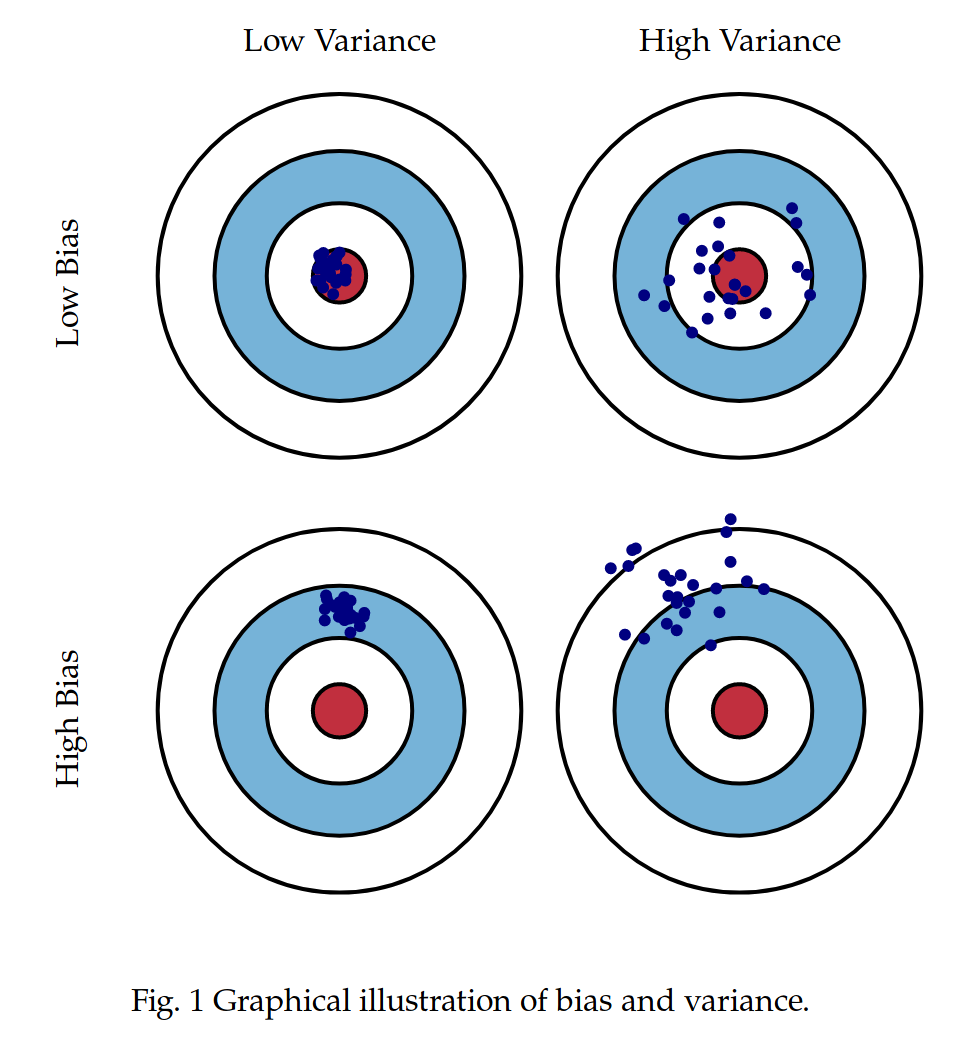
\includegraphics[width=0.5\linewidth]{Images/bias-variance-tradeoff.png}
    \caption{Bias Variance Tradeoff}
\end{figure}
\begin{figure}[H]
    \centering
    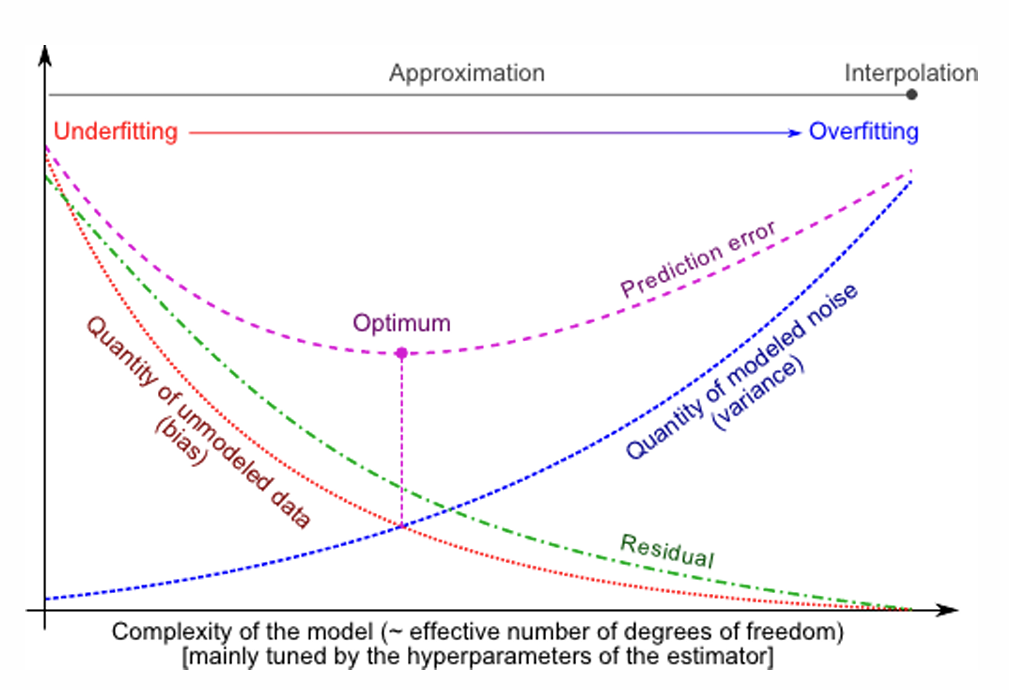
\includegraphics[width=0.5\linewidth]{Images/bias-variance-optimum.png}
    \caption{Bias Variance Tradeoff Optimum}
\end{figure}

\defn{Bias-Variance Summary}{
    In principle we say:
    \begin{itemize}
        \item \textbf{Flexible} methods have low bias but high variance
        \item \textbf{Simple} methods have low variance but high bias
    \end{itemize}
}
\begin{figure}[H]
    \centering
    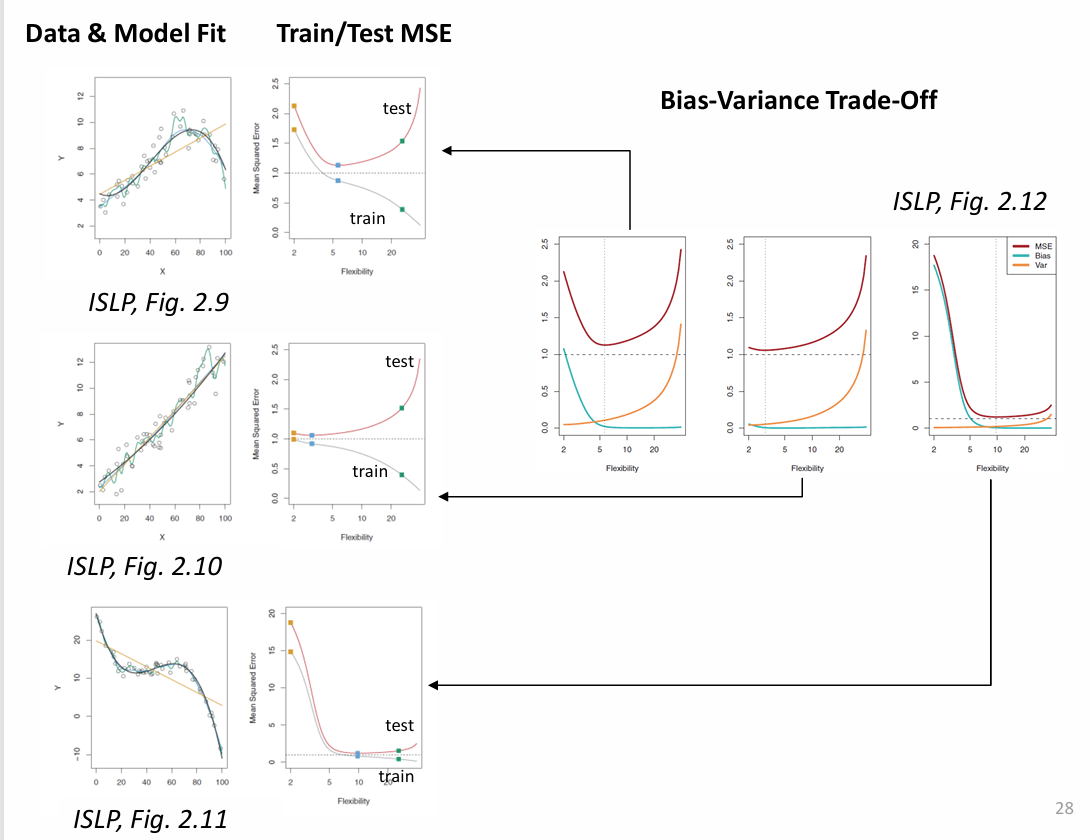
\includegraphics[width=1\linewidth]{Images/bias-variance-tradeoff-overview.png}
    \caption{Bias Variance Overview}
\end{figure}

\defn{Model Selection Merksatz}{
    Don't select the method minimizing the \textbf{training MSE}!
}

\newpage
\section{Regression}
\begin{figure}[H]
    \centering
    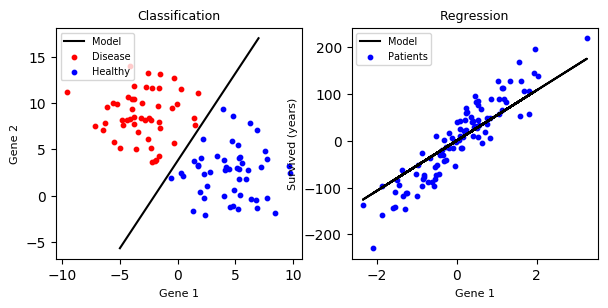
\includegraphics[width=0.5\linewidth]{Images/regr-vs-class.png}
    \caption{Regression vs Prediction}
\end{figure}
Regression is a method to calculate \textbf{quantitative} (numerical) predictions where \(Y\) is an ordered numerical value.
In its essence we define a mathematical model and an associated error function.
We then try to minimize the error, which is \textit{just} an optimization problem.

For a model to be optimizable many different well known optimization models exist.
For most regression problems we use \textbf{RSS}.
With the RSS we try to minimize the difference between squared sums of the prediction \(\hat{Y}\) and the actual data \(Y\).

The terms are squared to keep a positive sign. It can also be modeled with the abs function, 
but this makes it harder to find an optimization method due to it beeing harder to be optimized using analysis e.g. differentiation.
\defn{RSS}{
    \begin{equation}
        RSS = \sum (y - \hat{y})^2
    \end{equation}
}

\subsection{Model Accuracy}
We can model the accuracy of a model using the \textbf{MSE}.
In essence the MSE shows the on average commited error when predicting already known values.

\defn{Mean Squared Error}{
    \begin{equation}
        \begin{split}
            MSE &= \frac{1}{n}(y_i-\hat{f}(x_i))^2 \\
            MSE &= \frac{RSS}{n}
        \end{split}
    \end{equation}
}

\newpage
\section{Linear Regression}
In linear regression estimates are modeled with a linear relationship between a scalar response (dependent variable) 
and one or more explanatory variables (regressor or independent variable). There is a closed form solution for the RSS optimization.
\defn{Linear Regression Model}{
    We use a linear model (linear in \(b_i\)):
    \begin{equation}
        Y \approx \hat{Y} = \beta_0 + \sum_{i=0}^n \beta_{i+1} X_i
    \end{equation}
    \(b_0\) is also called a bias term.
    We find a optimal prediction function by minimizing the RSS:
    \begin{equation}
        RSS = e_1^2+\dots+e_n^2 \text{ where } e_i = y_i-\hat{y}_i
    \end{equation}
}

\defn{Coefficients in Simple Linear Regression}{
    \begin{equation}
        \begin{split}
            \hat{b}_1 &= \frac{\sum_{i=1}^{n} (x_i - \bar{x})(y_i - \bar{y}) }{\sum_{i=1}^{n} (x_i - \bar{x})^2} \\
            \hat{b}_0 &= \bar{y} - \hat{b}_1 \bar{x}
        \end{split}
    \end{equation}
}

\subsection{Metrics}
\textbf{RSE} is roughly speaking, the average amount that the response will deviate from the true regression line. It provides an absolute measure of lack of fit of the model to the data. In fact the RSE carries the same unit as \(Y\).\textbf{ \(R^2\)} is the proportion of the variance explained by the model and hence it takes values between 0 and 1. \textbf{TSS} is the total sum of squares, which is the RSS if \(Y\) would always be predicted using the sample mean of \(Y\) (best possible predictor if we do not measure \(X\)). Assess accuracy of model with:
\defn{Model Accuracy}{
    \begin{equation}
        \begin{split}
            RSE &= \sqrt{\frac{1}{n-p-1}RSS} \\
            TSS &= \sum (y_i - \bar{y} )^2 = n \sigma_Y^2\\
            R^2 &= \frac{TSS-RSS}{TSS} = 1-\frac{RSS}{TSS} \\
        \end{split}
    \end{equation}
}

Since RSE includes the predictor count in the denominator it punishes adding more predictors to the model.
In TSS adding more predictors is always improving the metric.
\textbf{In simple linear regression} the following holds:
\begin{equation}
    R^2 = Cor(X,Y)^2 = Cor(Y,X)^2
\end{equation}
\textbf{In multivariate linear regression} the following holds:
\begin{equation}
    R^2 = Cor(Y,\hat{Y})^2
\end{equation}
We require a small variance of the estimate or equivalently a small standard error. Since \(\sigma^2\) is unknown it has to be estimated from data. Note that \(\sigma\) is the standard deviation of each independent realization of \(Y\).
\begin{equation}
    \begin{split}
         Var(\hat{\mu}) = SE(\hat{\mu})^2 = \frac{\sigma^2}{n}\\
         \text{where } \sigma^2 = Var(\epsilon)
    \end{split}
\end{equation}
Variance \(\sigma^2\) estimation using residual standard error (RSE):
\defn{Standard Error Estimation using RSE}{
    \begin{equation}
    \begin{split}
        \text{for }\sigma^2 &= Var(\epsilon) \\
        \implies SE\approx  \hat{SE} = RSE &= \sqrt{\frac{1}{n-p-1}RSS}
    \end{split}
\end{equation}
}

\subsection{Predictor Correlation}
There is a common effect in practice, where in simple linear regression a predictor is significant (has a low p-value)
but is insignificant in multiple linear regression.
This can happen when there is a latent variable, which is correlated with two other variables.

When the other two variables are 
regressed onto each other, it appears 
that there is a relationship between 
them, even though the both depend 
on the same latent variable.

\defn{Correlation (Empirical)}{
    \begin{equation}
        Cor(X,Y) = \frac{\sum (x_i - \bar{x}) (y_i - \bar{y})}{\sqrt{\sum (x_i - \bar{x})^2} \sqrt{\sum (y_i - \bar{y})}}
    \end{equation}
    Here x and y does not denote dependent or independent variables but any two random variables e.g two predictors.
}

The correlation values are best interpretable in a normalized correlation matrix:
\begin{figure}[H]
    \centering
    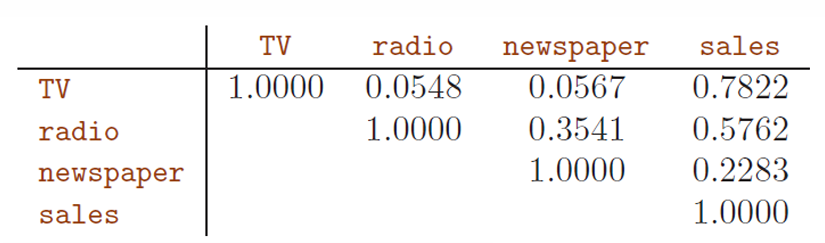
\includegraphics[width=0.5\linewidth]{Images/corr-example.png}
    \caption{Normalized Coeff Correlation Example}
\end{figure}

\subsection{Prediction Errors}
\defn{Errors in Prediction}{
    When predicting values we have three possible errors:
    \begin{enumerate}
        \item Inaccuracy in estimating the coefficients (Use confidence intervals)
        \item Model bias (Assume linear model fits good enough)
        \item The irreducible error \(\varepsilon\) (Prediction interval)
    \end{enumerate}
}

Confidence intervals quantify the uncertainty surrounding the averages of a prediction.
Here we are not interested in the overall \(\varepsilon\), since it does not contribute to the uncertainty
in the confidence interval. This is because \(\varepsilon\) is zero in the linear model.
If you can afford to average over many take confidence intervals otherwhise choose prediction invervals

\exm{Confidence vs Prediction Intervals}{
    \begin{itemize}
        \item Confidence interval = 95\% \textbf{of all data samples} lie in that interval.
        \item Prediction interval = with 95\% chance, the true value \(y\) of \textbf{one data sample} lies in that interval
    \end{itemize}
}

Under the Gaussian assumption confidence intervals can be computed using the estimated variance. 
\defn{Confidence Intervals}{
    \begin{equation}
    Pr(a<\hat{b}_i<b)=0.95 \implies \hat{\beta}_i \pm 2\cdot \hat{SE}(\hat{\beta}_i)
\end{equation}
}

\subsection{Predictor Selection}
\begin{itemize}
    \item Forward selection
    \item Backward selection
    \begin{itemize}
        \item Cannot be used if there are more predictor variables than training samples
    \end{itemize}
    \item Mixed Selection
\end{itemize}

\subsection{Assessing Coefficients: T-Test}
The T-test (with the T-statistic), is a tool for evaluating the means of one or two populations using hypothesis testing) Hypothesis tests using null hypothesis. We can test the relevance of coefficients using the T-test:
\defn{T-Test for Coefficients}{

\begin{equation}
    \begin{split}
        H_0 : \text{There is no relation between }X \text{ and }\\
        \text{or } b_i = 0 \\
        H_a : \text{There is a relationship}
    \end{split}
\end{equation}
\begin{equation}
    \text{T-statistic} = \frac{\hat{\beta}_i}{\hat{SE}(\hat{\beta}_i)}
\end{equation}
With \(n-n_\beta\) degrees of freedom where p:
\begin{equation}
    p = Pr(|T|>|t| \qquad | H_0)
\end{equation}
}
\textbf{P-Value} is the probability that we realistically observe an absolute T-value equal or bigger to the one observed under the \(H_0\).

\subsection{Assessing Coefficients: F-Test}
An F-test is any statistical test used to compare the variances of two samples or the ratio of variances between multiple samples. To check if there is any relationship between predictors and the dependent variable the F-test can be used:
\defn{F-Test}{
    \begin{equation}
    \begin{split}
        H_0 &: \beta_0 = \dots = \beta_n = 0 \\
        H_a &: \text{at least one } \beta_j \text{ is non-zero} \\
        \text{using F-statistic} &: \frac{\text{explained variance}/p}{\text{unexplained variance}/(n-p-1)} \\
        \text{using F-statistic} &: F=\frac{(TSS-RSS)/p}{RSS/(n-p-1)}\\
        \text{and} &: TSS = \sum (y_i-\bar{y})^2 = n\sigma^2 \text{, } RSS=\sum (y_i - \hat{y})^2
    \end{split}
\end{equation}
}
F-statistic expresses the improvement of the model per parameter \(p\) in multiples of the residual variance. If the linear model assumptions are correct and \(H_a\) is true we expect the F-statistic on average to be greater than one.

One can also use a subset of \(q\) coefficients to test with a new hypothesis. We order the predictor variables so that the last q variables are the one to test for being zero. Then we fit a second model that uses all the predictor variables except the last q .
\begin{equation}
    F = \frac{(RSS_0-RSS)/q}{RSS/(n-p-1)}
\end{equation}
\defn{Single Coefficient F-Test}{
    When we leave out only one variable (q=1) then the F-statistic would tell the partial effect of adding that variable to the model. \textbf{It turns out, the F-statistic, if only one variable is left out, is identical to the squared T-statistic.}
}

\begin{figure}[H]
    \centering
    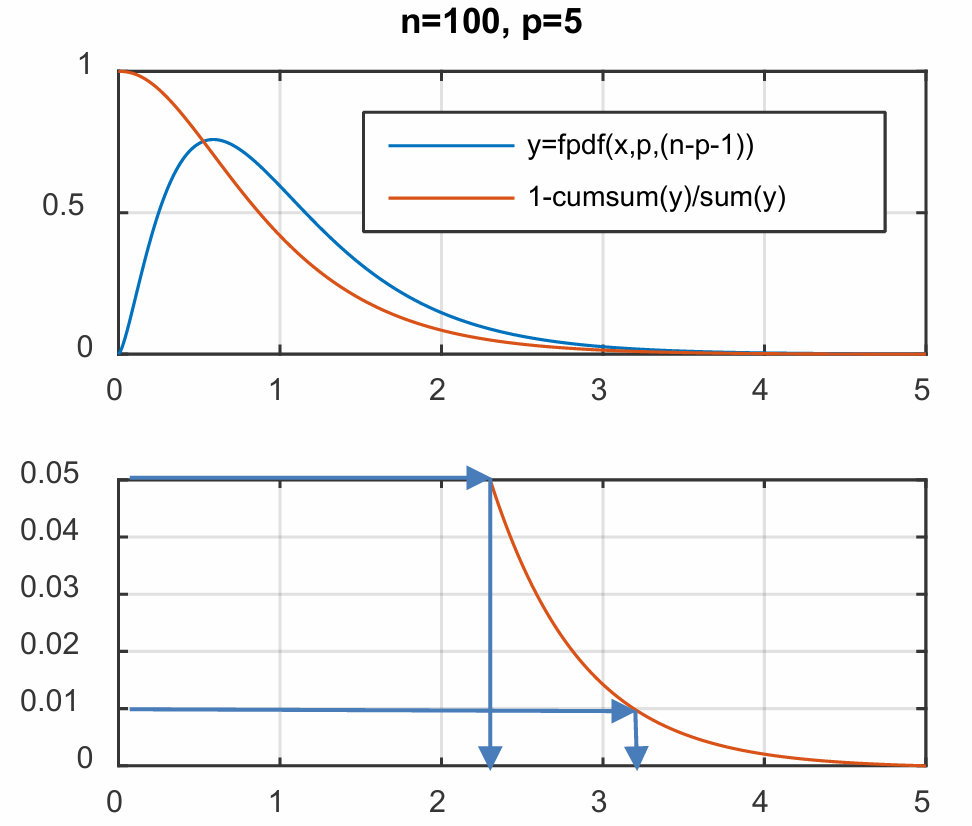
\includegraphics[width=0.5\linewidth]{Images/f-dist.png}
    \caption{F-Distribution}
\end{figure}

\subsection{Potential Problems}
\begin{enumerate}
    \item Non-linearity of data -> look at residual plots -> transform inputs
    \item Correlation of error terms -> caution when collecting data!
    \item Non-constant variance of error terms -> look at residual plots -> transform output
    \item Outliers (unusual output value) -> if \(\frac{\hat{\epsilon}_i}{\hat{\sigma}\sqrt{1-h_i}}>3\) -> outlier
    \item High-leverage points (unusual input value) -> if \(h_i = \frac{1}{n} + \frac{(x_i - \bar{x})^2}{\sum_{i=1}^{n} (x_i - \bar{x})^2} > (p+1)/n\) -> h.l.p
    \item Collinearity -> if \(VIF(\hat{b}_j) = \frac{1}{1-R_{X_j|X_{-j}^2}}>5\) -> problem
\end{enumerate}

\subsection{Qualitative Predictors}
Binary qualitative predictors can be modeled in linear regression using a technique that maps
the class to either 0 or 1 this is often called dummy or indicator variables:

\begin{equation}
    x_i = \begin{cases}
        1 & \text{if class x}\\
        0 & \text{if class y}
    \end{cases}
\end{equation}
The model can then be extended to:
\begin{equation}
    y_i = b_0 + b_1 x_1 + \varepsilon_i = \begin{cases}
        b_0 + b_1 + \varepsilon_i \\
        b_0 + \varepsilon_i 
    \end{cases}
\end{equation}
This simplifies into a linear function with slope influence or only with a bias term.

\begin{figure}[H]
    \centering
    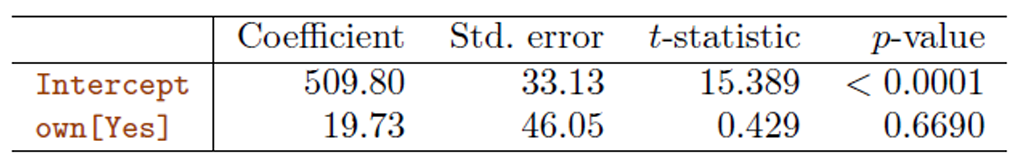
\includegraphics[width=0.75\linewidth]{Images/indicator-function.png}
    \caption{Dummy/Indicator Variable}
\end{figure}

If multiple qualitative predictors are to be modeled new dummy variables need to be introduced.
There always only needs to be \(l-1\) dummy variables where l is the number of levels. The level
without a dedicated dummy variable is called the baseline.

It is better to use the F-test to judge if the predictors are relevante,
since the individual p-values of the coefficients rely on the chosen encoding of the dummy variable. 

\subsection{Removing the additive assumption (Interaction Terms)}
The linear model assumes that the relationship between the predictors and the response are additive and linear.
Additivity implies that the change in the response due to a unit change in a predictor is independent of the value
of the other predictors.

\defn{Cross-Terms}{
    We can remove additivity by introducting cross-terms:
    \begin{equation}
        Y = b_0 + b_1 X_1 + b_2 X_2 + b_3 X_1 X_2 + \varepsilon
    \end{equation}
}

The hierarchical principle states, that if there is an interaction 
term in a model, then the two main effects should also be 
included even when their p-values are large.

\subsection{Non-linear relationships TBD}

\section{Polynomial Regression}
Is a straightforward extension to 
linear regression:
\defn{Polynomial Regression}{
    \begin{equation}
        y_i = b_0 + b_1 x_i + \dots + b_d x_i^d + \varepsilon_i
    \end{equation}

    Linear solvers will provide the covariance matrix:
    \begin{equation*}
        \hat{C} = Cov(\hat{b}_j)
    \end{equation*}

    The variance of the model is computed at a certain value \(x_0\)
    \begin{equation}
        \begin{split}
            Var[ \hat{f}(x_0)] &= l_0^T \hat{C} l_0 \\
            \text{With } l_0^T &= (1,x_0,\dots,x_n^d)
        \end{split}
    \end{equation}

    Polynomials (especially higher order ones) perform very bad at the \textbf{boundaries}.
    It is better to use Regression Splines. Polynomial Regression shall be used
    if the underlying function is "known".
}

\begin{figure}[H]
    \centering
    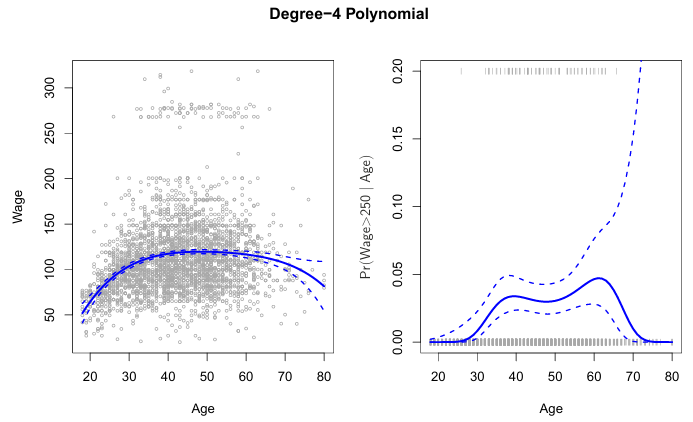
\includegraphics[width=0.75\linewidth]{Images/polynomial-regression.png}
    \caption{Polynomial Regression}
\end{figure}

Orders higher than 4 are 
uncommon, since this can result in very 
wiggly functions especially close to the 
boundaries of the X variable

\section{Step-Functions}
Step functions allow for local approximations by 
braking \(X\) into bins and fitting a different constant in each bin.
This amounts to converting a continuous 
variable \(X\) into an ordered categorical variable.

\begin{figure}[H]
    \centering
    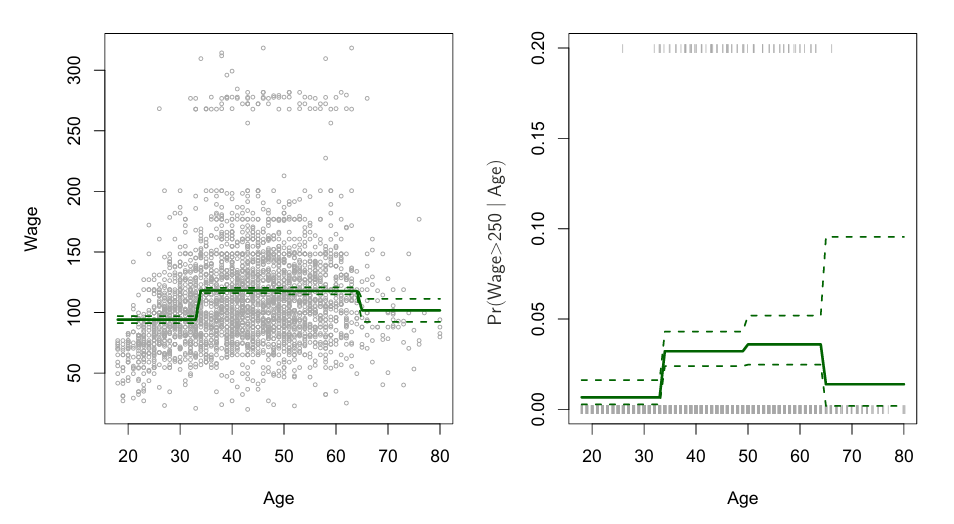
\includegraphics[width=0.75\linewidth]{Images/step-functions.png}
    \caption{Step Functions}
\end{figure}

\defn{Step-Function}{
    For a series of indicator functions:
    \begin{equation*}
        \begin{split}
            C_0(X) &= I(X < c_1) \\
            C_1(X) &= I(c1 \leq X < c_2) \\
            \vdots \\
            C_{K-1}(X) &== I(c_{K-1} \leq X < c_k) \\
            C_K(X) &= I(c_K \leq X) \\
            \text{For which } &C_0 +  \dots + C_K = 1
        \end{split}
    \end{equation*}
    With cut points (\(c_1,\dots, c_n\)) which is a hyperparameter.
    We use linear regression:
    \begin{equation}
        y_i = b_0 + b_1 C_1(x_i) + \dots + b_K C_K(x_i) + \varepsilon_i
    \end{equation}
    This results in a piecewise constant function.
}

\section{Basis Functions}
The basis functions approach is a combination of
the foundations of polynomial and step function regression.
We construct a model function where certain basis function are used.

\defn{Basis Function Approach}{
    We define a certain function e.g polynomial basis functions:
    \begin{equation}
        b_j(x_i) = x_i^j
    \end{equation}
    \textbf{The basis functions must be fixed and known.}
    The basis functions can be defined in certain intervals.
    Then again we use linear regression:
    \begin{equation}
        y_i = \beta_0 + \beta_1 b_1(x_i) + \dots + \beta_K b_K(x_i) + \varepsilon_i
    \end{equation}
}

\section{Regression Splines}

Regression Splines combine the local approach of 
basis function and the flexibility of 
polynomials by fitting low degree 
polynomials over different \(X\) regions.
The points, where the coefficients 
change are called \textbf{knots}.
Using more knots leads to more flexible fits.

\begin{figure}[H]
    \centering
    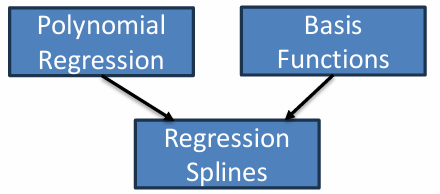
\includegraphics[width=0.4\linewidth]{Images/regression-splines.png}
    \caption{Regression Splines}
\end{figure}

\begin{figure}[H]
    \centering
    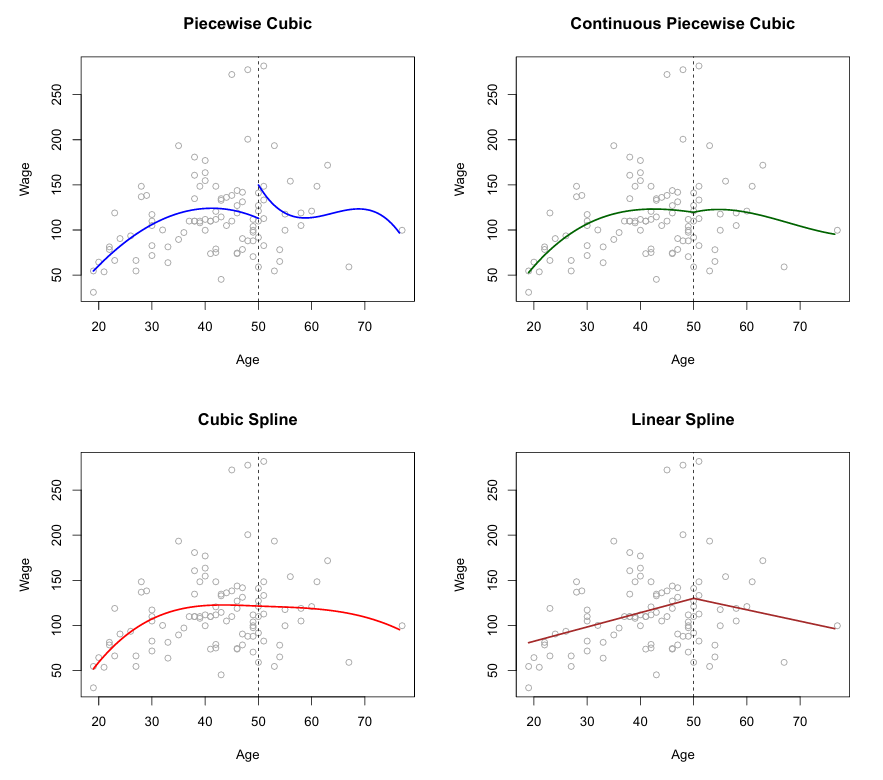
\includegraphics[width=0.75\linewidth]{Images/diff-regression-splines.png}
    \caption{Different Example of Regression Splines}
\end{figure}

\subsection{Constraints}
For splines to be smooth continues transitions at the knots,
we need to impose constraints:
\defn{Spline Contrains}{
    \begin{equation}
        \begin{split}
            f_j(x_k) &= f_k(x_k) \\
            f_j'(x_k) &= f_k'(x_k) \\
            f_j''(x_k) &= f_k''(x_k)
        \end{split}
    \end{equation}
    Imposing constraints removes a degree of freedome (DoF).
    The first polynomial where this makes sense is qubic.
}

\defn{Truncated Power Basis Function}{
    \begin{equation}
        h(x, \xi) = (x-\xi)_+^3 = \begin{cases}
            (x-\xi)^3 &\text{if } x>\xi \\
            0  &\text{otherwise}
        \end{cases}
    \end{equation}
    Where \(\xi\) is the knot. We shift the cubic polynomial with \(\xi\).
    The function will stay continuous and have continuous first and second derivatives.
    If we use \(h(x,\xi)\) we are \textbf{guaranteed to have matching constraints}.
}

\subsection{Cubic Splines}

\begin{figure}[H]
    \centering
    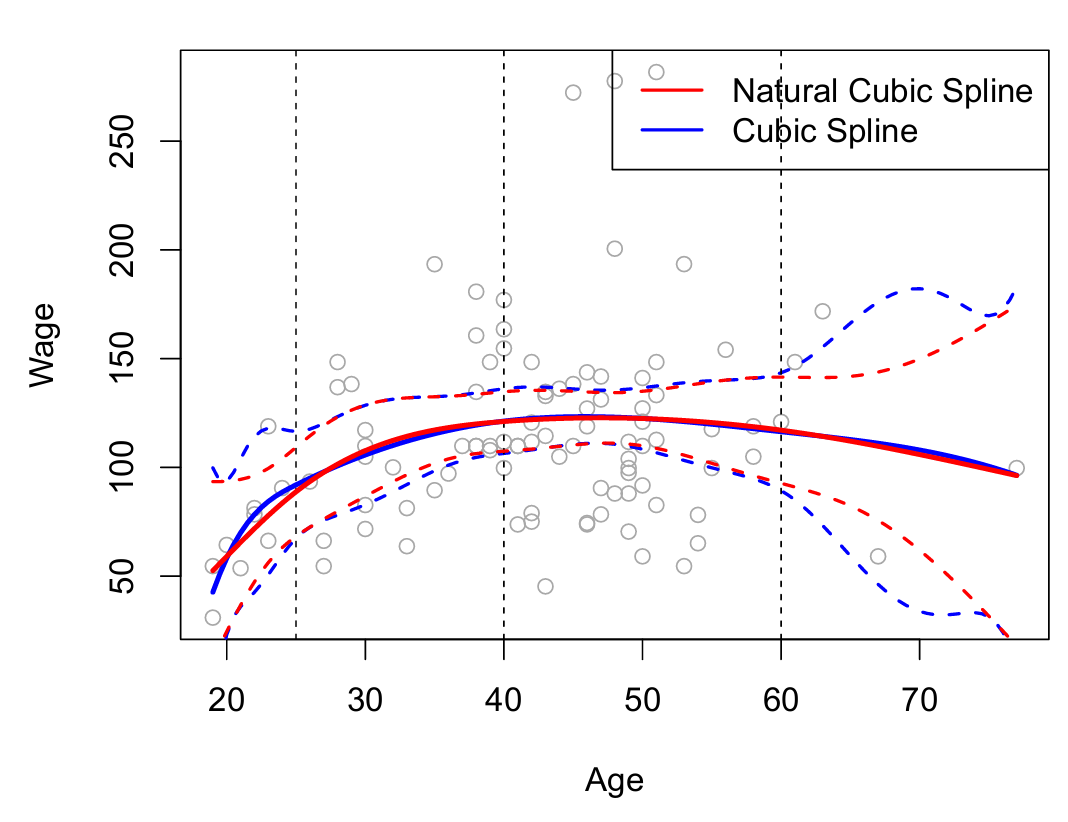
\includegraphics[width=0.5\linewidth]{Images/cubic-spline.png}
    \caption{Cubic Splines}
\end{figure}
\defn{Cubic Regression Splines}{
    In general, a cubic spline with K knots has \(K+4\) DOF.
    \begin{equation}
        y_i = b_0 + b_1 x_i + b_2 x^2_i + b_3 x^3_i + b_i h_k(x, \xi_k) + \varepsilon_i
    \end{equation}
}

\subsection{Natural Spline}
\defn{Natual Spline (Linear Boundaries)}{
    Since when using splines the boundaries have
    very big confidence intervals.
    We impose the further constraint,
    that the edges have to be linear.
    It has \((K+4)-4\) DOF.
    Natural splines perform immensively better at the boundaries
    compared to e.g. cubic regression splines.
}
Using a natural spline one can get more stable 
estimates at the boundaries as can be seen 
in the figure on the right, where the 
confidence interval of the natural spline is 
narrower and less wiggly than that of a 
cubic spline.

\subsection{Knot Selection}
\begin{multicols}{2}
    \begin{enumerate}
        \item Place them manually if you know the data.
        \item Place them at equal spacing. This is a bad approach if
        the data is not uniformly distributed.
        \item Do equal spacing on the histogram. E.g. space them
        at certain percentile of the data.
    \end{enumerate}
    The number of knots can be selected using cross-validation.
    
    \begin{figure}[H]
        \centering
        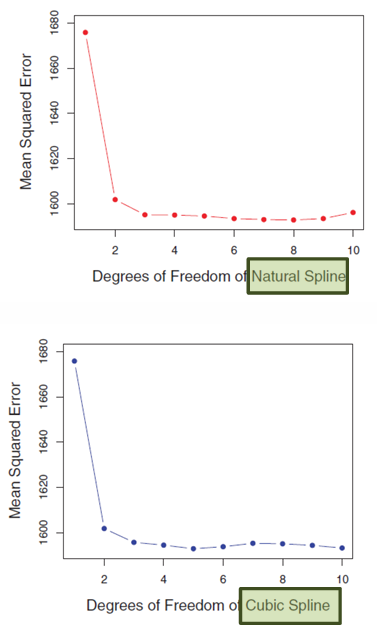
\includegraphics[width=0.75\linewidth]{Images/number-of-knots.png}
        \caption{Knot Count Selection}
    \end{figure}
\end{multicols}

\subsection{Smoothing Splines}

\begin{figure}[H]
    \centering
    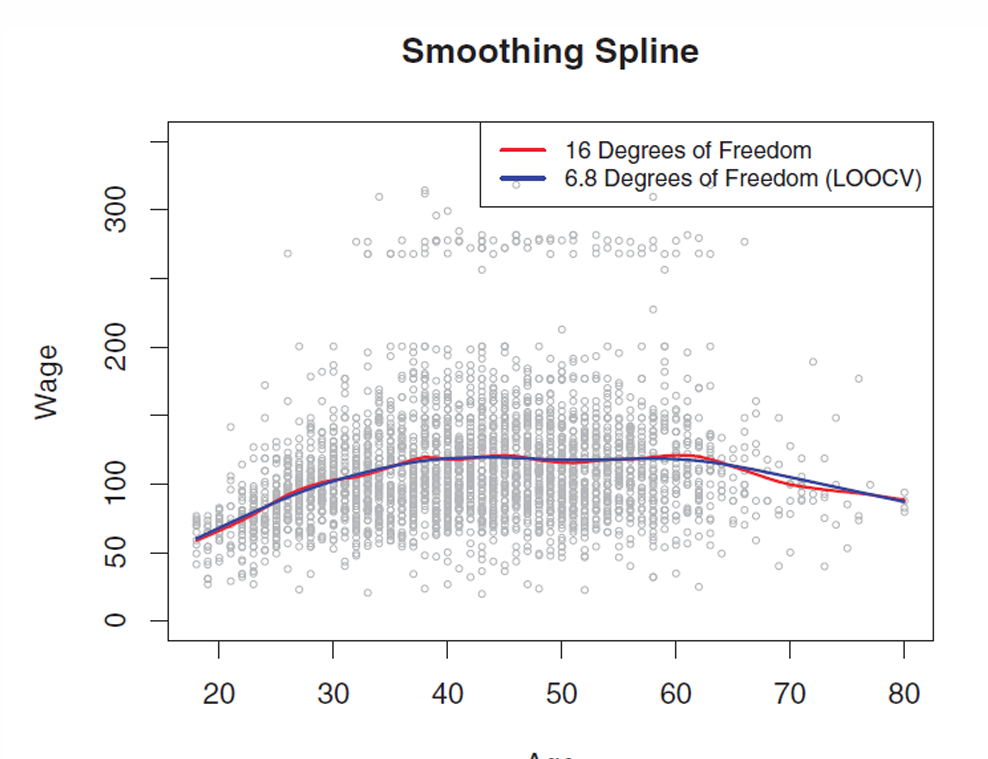
\includegraphics[width=0.5\linewidth]{Images/smoothing-spline.png}
    \caption{Smoothing Spline}
\end{figure}

When using smoothing splines one does not need to select the amount of knots
or the placement of the knots as hyperparameter.

When finding fitting our model:
\begin{equation*}
    \sum_{i=1}^{n} (y_i - g(x_i))^2
\end{equation*}
Where \(g(x_i)\) is any arbitrarily complex function,
we can impose restrictions on the roughness of the function,
so that it has less variance. For this we use the second
derivative, square it to make it positive and finally intergrate over it:
\begin{equation*}
    \int g''(t)^2 dt
\end{equation*}

\defn{Smoothing Splines}{
    Doesn't require pre-defined knots.
    We place a knot at every data sample \(x_i\) and regularize to enforce a smooth solution:
    \begin{equation}
        \sum_{i=1}^{n} (y_i - g(x_i))^2 + \lambda \int g''(t)^2 dt
    \end{equation}

    A smoothing spline is a natural cubic 
    spline with knots \textbf{at every unique 
    value of \(x_i\)}.

    There is a known equation for calculation the \textbf{effective degrees of freedome}
    which is a mapping from \(\lambda\). This makes it comparable to other regression methods.
    If you take the limit of \(\lambda = \infty\) the regression goes back to
    a line.
}
You almost always want to use smoothing splines, if using regression splines is beeing considered.

\section{Local Regression}

\begin{figure}[H]
    \centering
    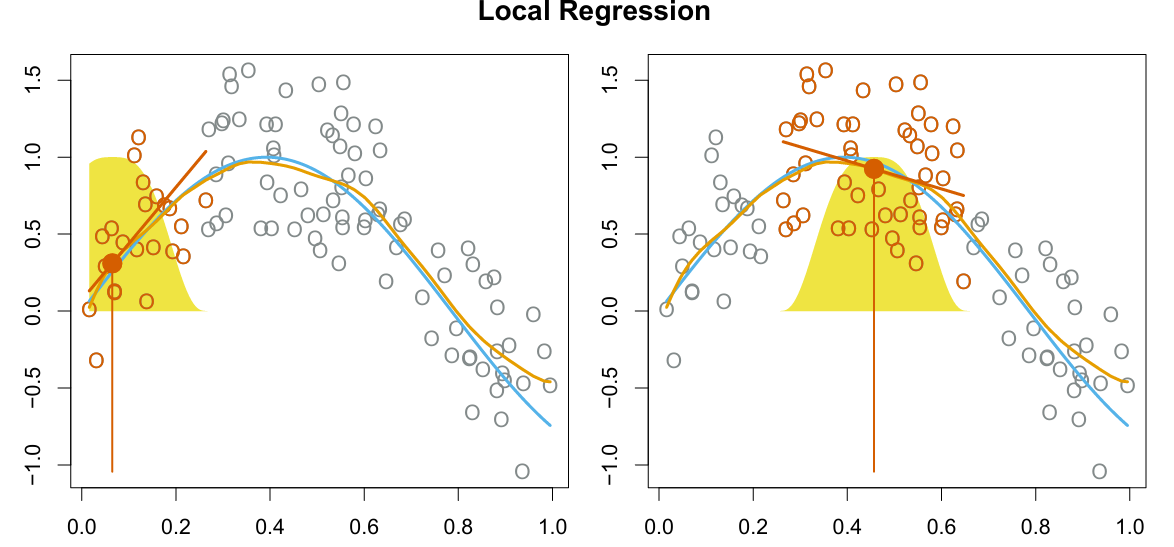
\includegraphics[width=0.75\linewidth]{Images/local-regression.png}
    \caption{Local Regression}
\end{figure}
\defn{Local Regression}{
    Fit a linear regression
    only to the data which
    is close to our test
    point \(x_0\).
    
    The nearest points are defined using a fraction of the total amount of points,
    this is called \textbf{span}:
    \begin{equation}
        span = \frac{k}{n}
    \end{equation}
    Often we also use another degree of freedome by introducing a weight to the nearest points
    e.g. using a gaussian (the bell in the figure).
    Using this method one can also compute the effective degrees of freedome.
}

Closeness is easy to define in low dimensions, but in high dimensions,
nothing is really close. This scheme only works well for \textbf{low dimensions}.
Computationally it is \textbf{not very efficient}.
For each new point we have to compute a linear regression.

\section{Generalized Additive Models}

Previous methods (Polynomial Regression, Regression Splines, Smoothing Splines and Local Regression) have been 
developed for a single predictor.
Generalized additive models (GAMs) extends these ideas to multiple predictors.
GAMs provide a framework for extending a linear model by allowing non-linear functions of each of 
the variables, while maintaining additivity. 

\defn{Additivity}{
    Additivity means that the effect of each predictor on the response variable is independent 
    of the other predictors. The contribution of a predictor and its coefficient does not modify 
    or depend on the effect of another predictor and its coefficient; their effects simply add up
    linearly in the model.
}

GAMs can be applied to quantitative and qualitative responses.

\defn{Generalized Additive Models}{
    \begin{equation}
        y_i = b_0 + \sum_{j=1}^{p} f_j(x_{ij})+\varepsilon_i
    \end{equation}
    We replace \(b_i x_i\) with some function \(f_i(x_i)\). It is important,
    that \(f_i(x_i)\) only depends on a single \(x_i\) so that additivity is kept.
    For \(f_i(x_i)\) we can use any available smooth function.

    For classification one can use a modified logistical approach:
    \begin{equation}
        \log(\frac{p(X)}{1-p(X)}) = b_0 + \sum_{j=1}^{p} f_j(X_{j})
    \end{equation}
}

For \(f_i(x_i)\) we could use for example: Linear Regression, Polynomial Regression, Regression Splines,
Smoothing Splines or Local Regression. These can be mixed and selected freely.

\subsection{Pros}
\begin{itemize}
    \item Easy method to fit non-linear functions in a linear regression framework.
    \item High predictive power.
    \item Interpretability thanks to additivity.
\end{itemize}
\subsection{Cons}
\begin{itemize}
    \item Model is restricted to be additive.
    \item Interaction terms must be defined manually
\end{itemize}
Conclusion: GAM are a useful compromise between linear models and fully nonparametric models.

\newpage
\section{Classification}
In classification we make qualitative (categorical) predictions where \(Y\) is a discrete categorical value.
As in regression there are many methods to quantify the error.

\subsection{Model Accuracy}
One of the most general methods is to model error with the Classification Error Rate (CER):
\defn{Classification Error Rate}{
\begin{equation}
    Error = \frac{1}{n}\sum_{i=1}^n I(y_i \ne \hat{y}_i)
\end{equation}
}

\subsection{Model Accuracy with Confusion Matrix}
\begin{figure}[H]
    \centering
    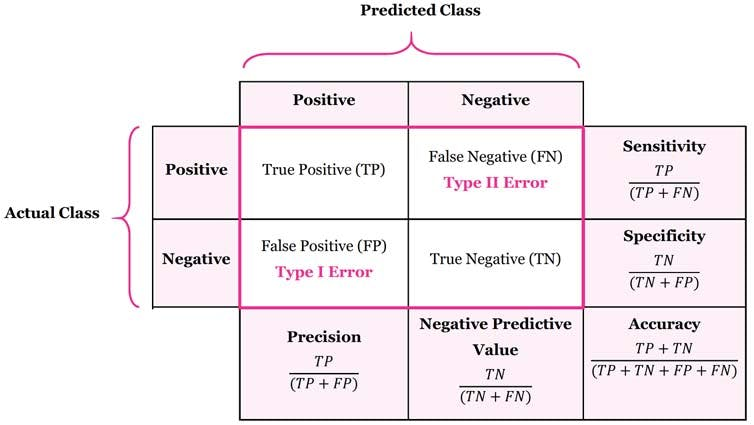
\includegraphics[width=0.75\linewidth]{Images/conf-matrix.jpg}
    \caption{Confusion Matrix}
\end{figure}

\subsection{Threshold selection using ROC}
receiver operating characteristic curve, or ROC curve,
is a graphical plot that illustrates the performance of a binary classifier model
(can be used for multi class classification as well) at varying threshold values.

\begin{figure}[H]
    \centering
    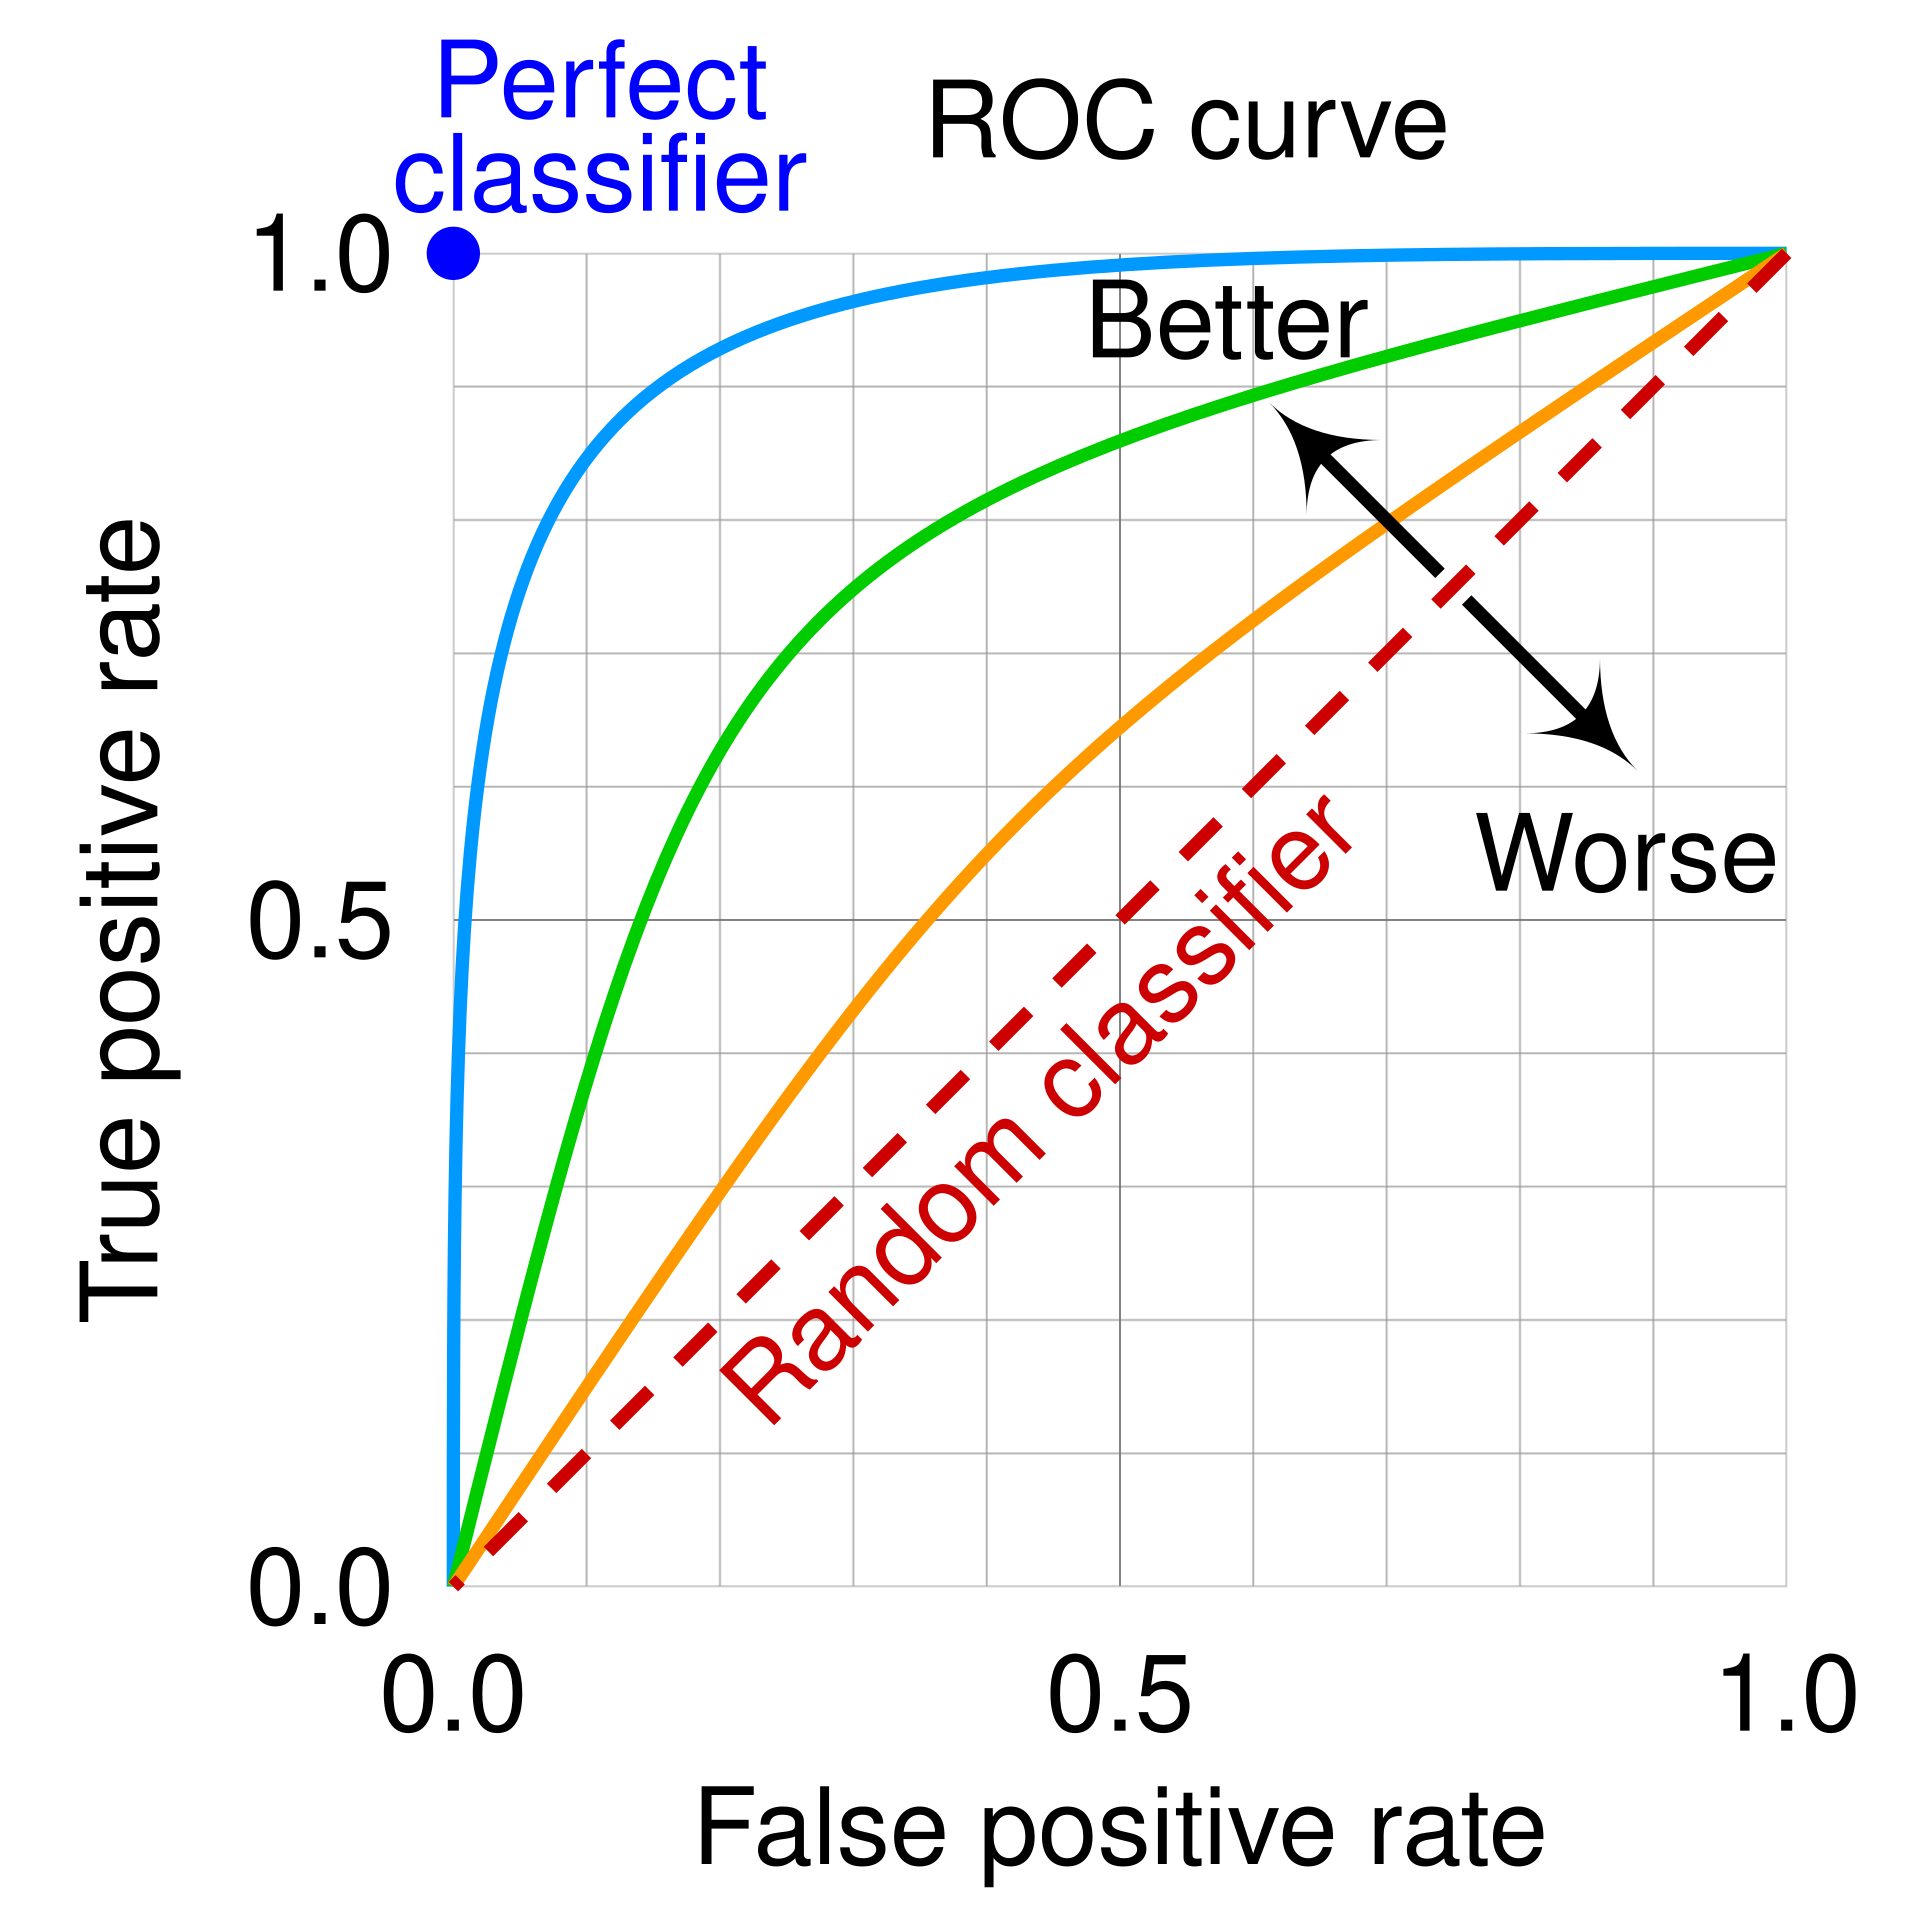
\includegraphics[width=0.5\linewidth]{Images/roc.png}
    \caption{ROC Graph}
\end{figure}

It is a graph that plots the true 
positive rate (TP/P) as a function of 
the false positive rate (FP/N).
Each binary classification scheme has 
a ROC, which is independent of the 
selected threshold.
The optimal curve hugs the left upper 
corner and is non-decreasing.
Hence the \textbf{area under the curve (AUC)} is a 
good measure for the fundamental 
performance of a binary classification 
scheme.

\defn{Important Terms}{
    \begin{description}
        \item[Sensitivity] can you find, what you want
        \item[Specificity] can you find, what you don't want
    \end{description}
    Ideally both, sensitivity and specificity are 
    high. Sensitivity is also called Recall.
}
\subsection{Bayes-Classifier}
A Bayes classifier results in the lowest possible overall test error rate:
\defn{Bayes Classifier}{
    Test error rate is minimized, by a classifier that assigns each observation to the most probable class, given its predictor value. Results in the lowest possible error rate called Bayes error rate.
    \begin{equation}
        \begin{split}
            &Pr(Y=j|X =x_0)\\
            \text{set class to: }max_j(&Pr(Y=j|X=x_0))
        \end{split}
    \end{equation}
    Where \(j\) is the most probable class for a given input variable (predictor) \(X=x_0\). E.g for a 2 class model: \(Pr(Y=1|X=x_0)>0.5\)

    The bayes error rate is analogous to the irreducible error and is 0.1304.
}

\newpage
\subsection{KNN}
\defn{K-Nearest Neighbors}{
    Bayes classifier requires knowledge of the conditional distribution of \(Y|X\), in a real world problem this is never known. K-nearest neighbors is the simplest of such methods in which given a test point \(x_0\) KNN finds \(K\) neighbors and then estimates the class probabilities as the fraction of neighbors which belong to a particular class.

    \begin{equation}
        Pr(Y=j|X=x_0)=\frac{1}{K}\sum_{i\in N_0} I(y_i=j)
    \end{equation}
    Where \(N_0\) are the nearest neighbors to the point \(x_o)\).
    \begin{itemize}
        \item Small K results in high variance
        \item Big K results in high bias
        \item K controls the trade off
        \item \(\frac{1}{K}\) is a measurement of flexibility
    \end{itemize}
    
}
\begin{figure}[H]
    \centering
    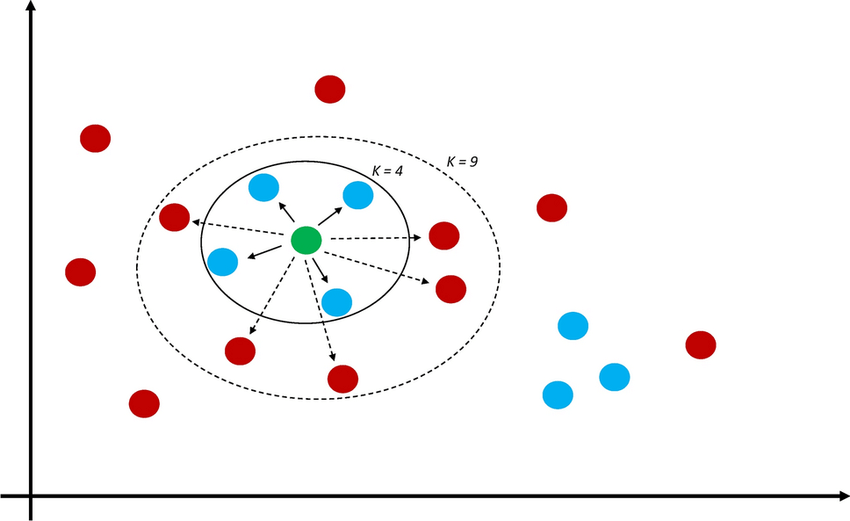
\includegraphics[width=0.75\linewidth]{Images/k-nearest.png}
    \caption{KNN}
\end{figure}

\begin{figure}[H]
    \centering
    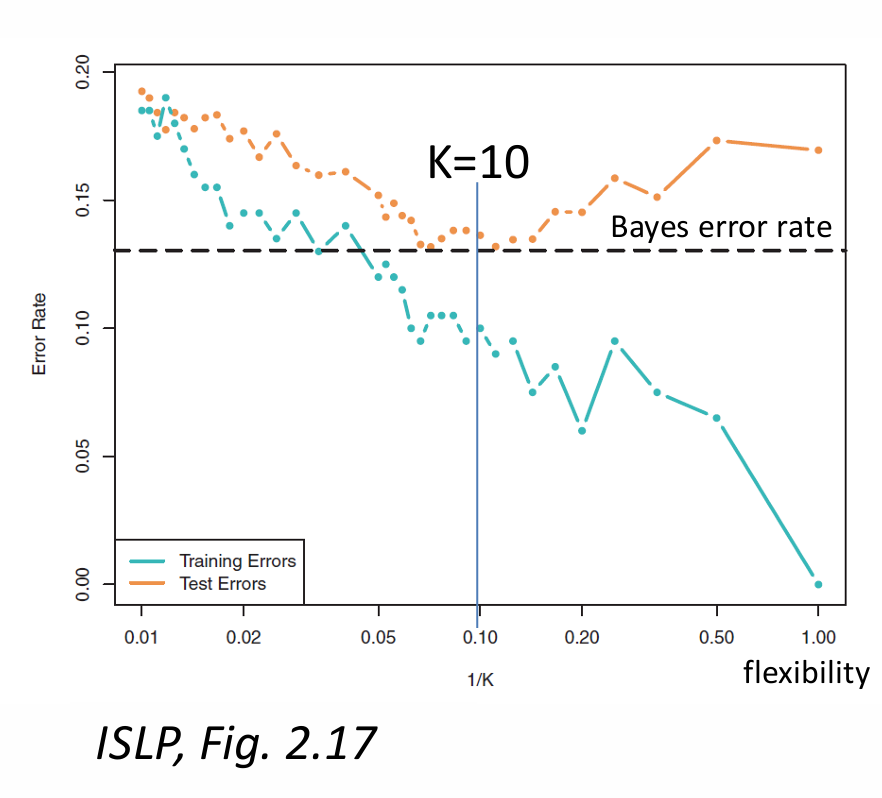
\includegraphics[width=0.5\linewidth]{Images/knn-flexibility.png}
    \caption{KNN Flexibility}
\end{figure}

\newpage
\subsection{Logistic Regression}
Linear regression does not work well for classification.
We instead use logistic regression where a probability [0;1] is modeled using:

 \begin{equation}
    \text{log odds } = log(\frac{p(X)}{1-p(X)}) = b_0 + b_1 X_1 + \dots + b_p X_p
 \end{equation}

 \defn{Logistic Regression}{
    \begin{equation}
        p(X) = \frac{e^{b_0 + b_1 X_1 + \dots + b_p X_p}}{1+ e^{b_0 + b_1 X_1 + \dots + b_p X_p}}
     \end{equation}
 }

 The parameters are found with the Maximum Likelihood approach, where we maximize:
 \begin{equation}
    l(b_0,b_1) = \prod_{i:y_i=1} p(x_i) \prod_{i':y_{i'}=0} (1-p(x_{i'}))
 \end{equation}

 \begin{figure}[H]
    \centering
    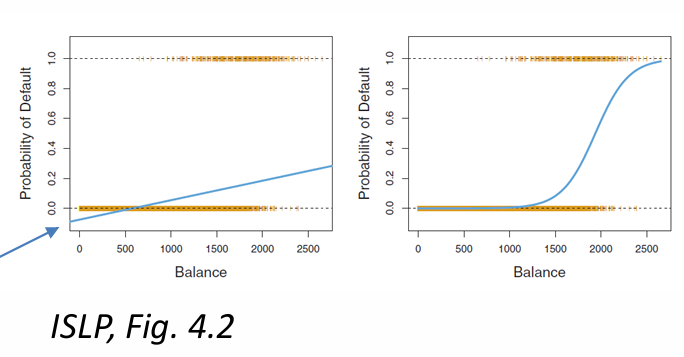
\includegraphics[width=0.75\linewidth]{Images/lin-reg-vs-log.png}
    \caption{Linear vs Logistic Regression}
\end{figure}

If we had three categories, we would 
need to estimate the probabilities of 
each of them, given the observed 
predictors.

Problems with Logistic Regression:
\begin{itemize}
    \item For well-separated classes: unstable results
    \item For small n: unstable results
    \item Workaround required for multiple classes
\end{itemize}

\subsection{Comparison of Methods}
\begin{multicols}{2}
    \subsubsection{Logistic Regression vs LDA}
    \begin{itemize}
        \item They often have very similar 
        performance 
        \item LDA tends to outperform logistic 
        regression if the Gaussian 
        assumption is approximately correct
        \item Logistic regression tends to 
        outperform LDA if the Gaussian 
        assumption is basically wrong
    \end{itemize}
    \subsubsection{KNN}
    \begin{itemize}
        \item  This is a non-parametric scheme, 
        hence no model is assumed
        \item Hence one would expect KNN to 
        outperform LDA and logistic 
        regression if the decision boundaries 
        need to be non-linear
        \item But KNN does not tell us which predictors 
        are important and need lots of training data
        \item Does not work at all in high dimensional 
        settings 
    \end{itemize}
    \subsubsection{QDA}
    \begin{itemize}
        \item In some sense this is a compromise 
        between simple linear boundaries of 
        LDA/logistic regression and arbitrary 
        boundaries of KNN
        \item Here the boundaries are 
        hyperparabolas, which are much 
        more complicated than hyperplanes 
        but still much less flexible than KNN 
        boundaries
        \item Hence it does take more training data 
        than the linear methods but much 
        less than KNN to perform well
    \end{itemize}
\end{multicols}

\newpage
\section{Classification with Linear Discriminant Analysis}
\subsection{With p=1}
In logistic regression: we directly 
model the probability \(P(Y | X)\).

In linear discriminant analysis we go 
the other way around, we estimate 
the probability density functions 
(pdf's) of the observations \(X\), given a 
particular class Y: i.e., \(p(X|Y)\)


If we model these pdfs as Gaussian, we 
result in a scheme very similar to logistic 
regression.


Then we apply Bayes' theorem to flip 
these probabilities around and get 
the ones on the top right, which 
allow us to make an optimal decision.

\begin{equation}
    P(Y|X) = \frac{P(X|Y)P(Y)}{P(X)}
\end{equation}

This is done by introducing the following new variables:
\begin{equation*}
    \begin{split}
        \pi_k &\quad \text{prior probability for class }k\\
        f_k(X) &\quad \text{pdf of } X \text{ for a class } k
    \end{split}
\end{equation*}
We then insert them:
\begin{equation*}
    P(Y=k|X=x) = \frac{\pi_k f_k(x)}{\sum_{l=1}^{K} \pi_l f_l(x)}
\end{equation*}

Estimating the prior probabilities \(\pi_k\) is 
straight forward. Simply use the fraction of samples in the 
training set that belong to class \(k\) as the 
estimate of the prior probabilities:
\begin{equation*}
    \pi_k = \frac{n_k}{n}
\end{equation*}

Estimating \(f_k(X)\) is more challenging.
In absence of any additional information, we use a Gaussian with different mean \(\mu_k\) and same variance \(\sigma_k^2\):
\begin{equation*}
    f_k(x) = \frac{1}{\sqrt{2\pi}\sigma_k} exp(-\frac{1}{2\sigma_k^2} (x - \mu_k)^2)
\end{equation*}

We further simplify the model by 
assuming that all \(k\) classes have the 
\textbf{same variance}. Hence:
\begin{equation*}
    \sigma_k^2 = \sigma^2
\end{equation*}

We can simplify this expression \(P(Y=k|X)\) to \(\varphi_k(x)\):
\begin{equation}
    P_k(x) = x \frac{\mu_k}{\sigma^2} - \frac{\mu_k^2}{2\sigma^2} + log(\mu_k)
\end{equation}

For two classes we could construct a new decision boundary:
\begin{equation*}
    f_b(x) = P_1(x)-P_2(x)
\end{equation*}
This could indicate class 1 for values greater than zero, class 2 for values smaller than zero and
the boundary line where the probabilities are equal.
This can be reformed to the decision boundary of:
\begin{equation*}
    x = \frac{1}{2} (\mu_1+\mu_2)
\end{equation*}
If the observation x falls exactly between the 
means of the two classes, then it could 
belong equally well to either class.

\begin{figure}[H]
    \centering
    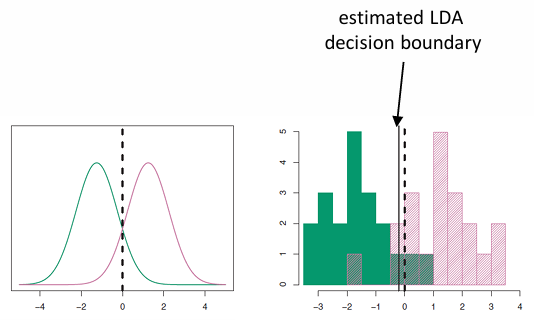
\includegraphics[width=0.75\linewidth]{Images/lda-decision-boundary.png}
    \caption{LDA Decision Boundary}
\end{figure}

\defn{LDA with p=1}{
The LDA method approximates the 
Bayes classifier by assuming Gaussian 
pdfs and using the following 
estimates for the means and the 
common variance.

\begin{equation}
    \begin{split}
        \hat{\mu}_k &= \frac{1}{n_k} \sum_{i:y_i=k} x_i \\
        \hat{\sigma}^2 &= \frac{1}{n-K} \sum_{k=1}^{K} \sum_{i:y_i=k} (x_i - \hat{\mu}_k)^2 \\
        \hat{\pi}_k &= \frac{n_k}{n} \\
        P_k(x) &= x \frac{\mu_k}{\sigma^2} - \frac{\mu_k^2}{2\sigma^2} + log(\mu_k)
    \end{split}
\end{equation}

Pick theclass with the largest \(P_k\)
}

\newpage
\subsection{Multiple Predictors p>1}
Extending LDA to multiple predictors 
results in the need for a model of a 
multidimensional pdf.

We will select a multidimensional 
Gaussian pdf where the means of the 
classes are different but all classes 
have the same covariance matrix.

\defn{Covariance Matrix}{
    Variance is defined as:
    \begin{equation}
        var(X) = E\{(x-\mu)^2\}
    \end{equation}
    In or more formally:
    \begin{equation*}
        var(X) = E(X^2)-E(X)^2
    \end{equation*}
    In multidimensional cases, this is the covariance matrix:
    \begin{equation}
        \Sigma = E\{ (x- \mu )(x -\mu)^T \}
    \end{equation}

    Since the correlation coefficient \(p_{ij}\) is given by:
    \begin{equation}
        p_{ij} = \frac{\sigma_{ij}}{\sigma_i \sigma_j}
    \end{equation}
    The matrix can thus be written as e.g:
    \begin{equation}
        \Sigma = \sigma_1 \sigma_2 \begin{bmatrix}
            \frac{\sigma1}{\sigma_2} & p_{12} \\
            p_{12} & \frac{\sigma_2}{\sigma_1}
        \end{bmatrix}
    \end{equation}
    Here \(x\) is a vector of observations.
    \(\mu\) is the mean vector, where each class has its own mean vector \(\mu_k\).
    \(\Sigma\) is the \(pxp\) covariance matrix that is common to all the classes.
}

After some algebra, a similar 
discriminant formula results in the 
multidimensional LDA as in the one
dimensional one:
\defn{Multidimensional LDA}{
    \begin{equation}
        \begin{split}
            \hat{\mu}_k &= \frac{1}{n_k} \sum_{i:y_i=k} x_i \\
            \hat{\Sigma} &= \frac{1}{n-K} \sum_{k=1}^{K} \sum_{i:y_i=k} (x_i - \hat{\mu}_k) (x_i - \hat{\mu}_k)^T \\
             \hat{\pi}_k &= \frac{n_k}{n} \\
             P_k(x) = x^T \Sigma^{-1} \mu_k - \frac{1}{2} \mu_k^T \Sigma^{-1} \mu_k + \log \pi_k
        \end{split}
    \end{equation}

    With little training data use LDA, otherwise QDA.
}

\begin{figure}[H]
    \centering
    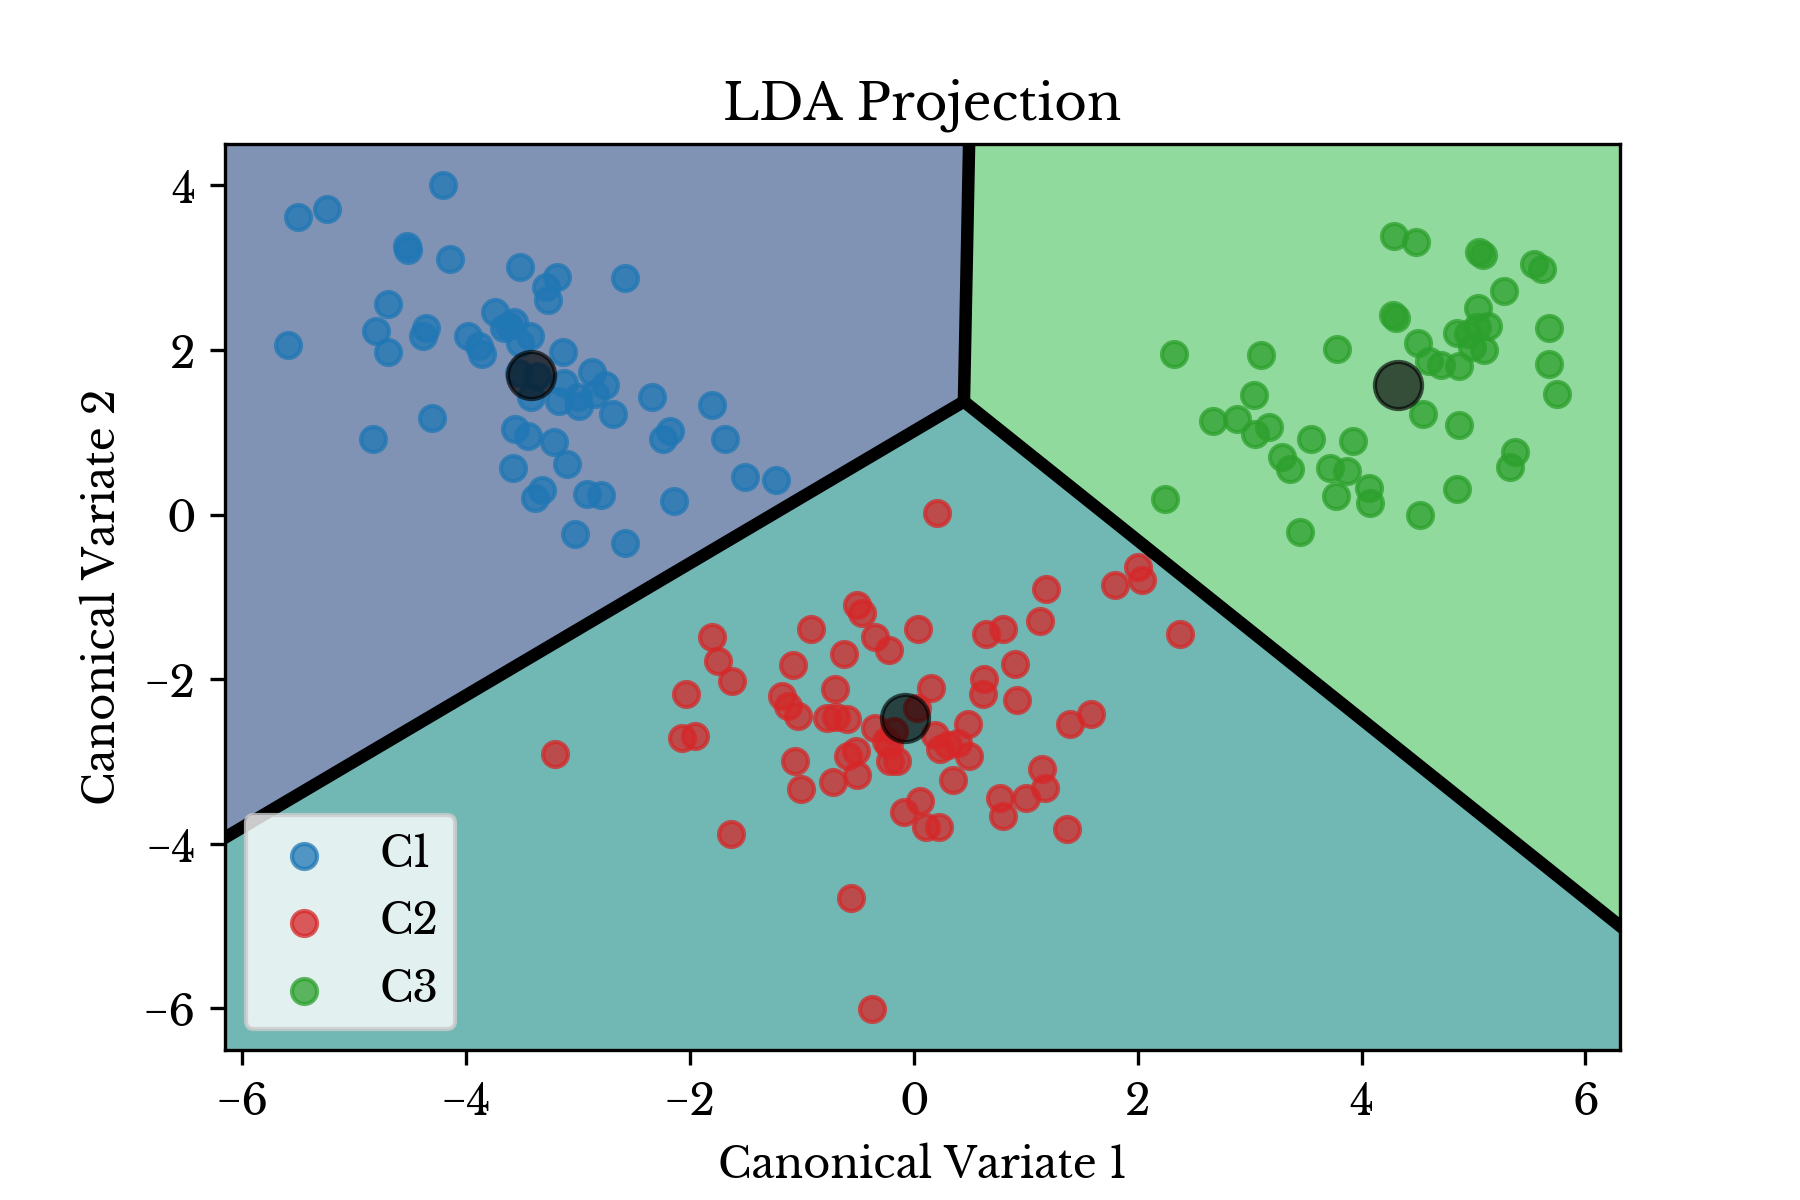
\includegraphics[width=0.75\linewidth]{Images/lda-dec-boundary.png}
    \caption{LDA Decision Boundary}
\end{figure}

\begin{figure}[H]
    \centering
    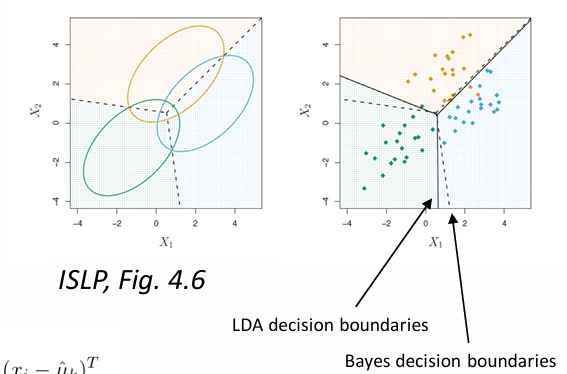
\includegraphics[width=0.75\linewidth]{Images/lda-dec-boundary-2.png}
    \caption{LDA Decision Boundary}
\end{figure}

\subsection{Error Intepretation}
In LDA the goal is 
to approximate a Bayes classifier which is 
optimized for minimum overall error rate.
Minimizing the overall error rate is not always the desired goal.

We can vary the threshhold to vary the error rate. We can use ROC
to find an optimal threshold.

\newpage
\section{Classification with Quadratic Discriminant Analysis}

Quadratic discriminant analysis (QDA) 
allows for each class to have its \textbf{own
covariance matrix}.
The fundamental effect is, that the 
discriminant functions per class for a 
given observation \(x\) changes to 
include a \textbf{new quadratic term}.

\begin{figure}[H]
    \centering
    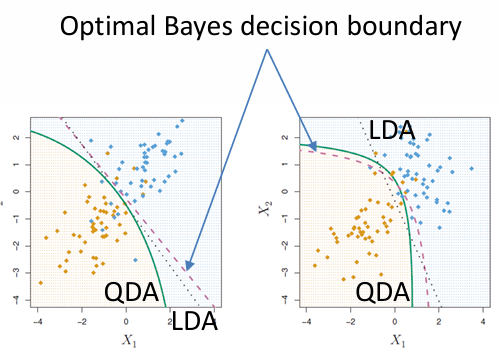
\includegraphics[width=0.75\linewidth]{Images/qda-vs-lda.png}
    \caption{QDA vs LDA}
\end{figure}

\defn{QDA}{
    Assumption:\( p(x|y=k)\) is Gaussian, where eachclass \(k\) has its
    own mean vector \(\mu_k\) and each class has its own covariance matrix \(\Sigma_k\).

    \begin{equation}
        P_k(x) = - \frac{1}{2} x^T \Sigma_k^{-1} (x - \mu_k) - \frac{1}{2} \log |\Sigma_k| + \log \pi_k
    \end{equation}

    QDA has more parameters than LDA thus increasing variance and decreasing bias.
    The QDA is quadratic in \(x\) since each class has its own covariance matrix hence the boundaries are hyperparapolas.
    With little training data use LDA, otherwise QDA.
}
\newpage

\section{Resampling Methods}
These are methods which use the given training 
set over and over again, this is achieved by sampling that set, i.e., 
create different subsets. To each of these subsets, the model 
can be fitted which allows for a statistical evaluation of the fitting.
Resampling is especially useful when:
\begin{itemize}
    \item Data is limited and needs to be reused for training and evaluation.
    \item Uncertainty estimation is critical, such as in scientific studies or risk-sensitive applications.
    \item Model assessment and comparison are needed.
    \item Reducing overfitting and improving generalization are priorities.
\end{itemize}

\subsection{Cross-Validation}
Cross-validation can be used to estimate 
the test error in order to evaluate the 
performance of a method and finding an 
optimal flexibility setting (i.e., optimal hyperparameters).

\begin{figure}[H]
    \centering
    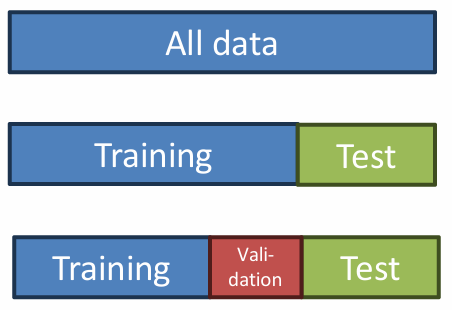
\includegraphics[width=0.25\linewidth]{Images/cross-validation.png}
    \caption{Cross-Validation}
\end{figure}

The basic idea is to hold out some samples from the 
training set and use these as a test set at the end, to 
estimate the final performance.

\begin{figure}[H]
    \centering
    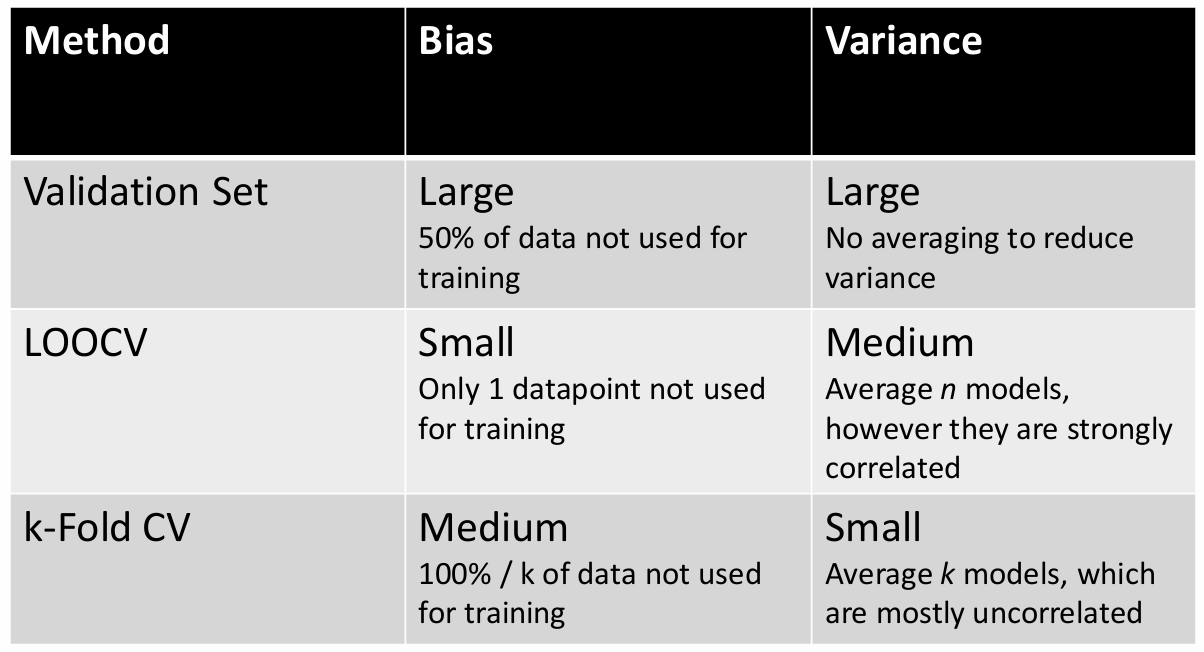
\includegraphics[width=0.75\linewidth]{Images/cross-val-comparison.png}
    \caption{Cross-Validation Comparison}
\end{figure}

\begin{figure}[H]
    \centering
    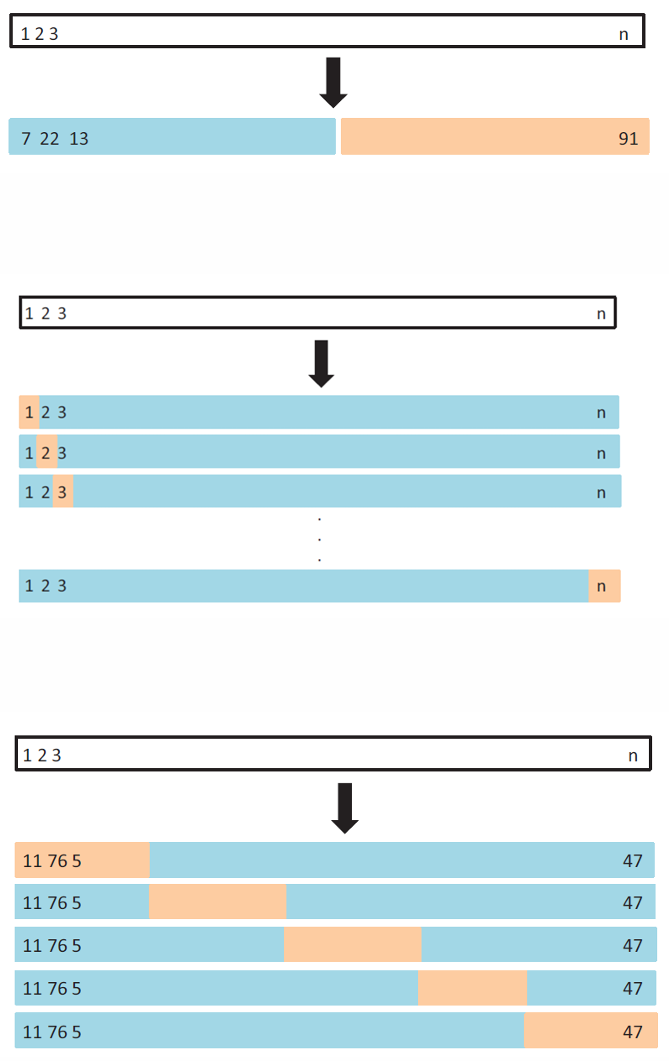
\includegraphics[width=0.5\linewidth]{Images/different-cross-validation-methods.png}
    \caption{Different Cross Validation Methods}
\end{figure}

\begin{multicols}{2}

    \subsection{Validation Set Approach} 
    The given observations are randomly 
    split into a training set and a 
    validation set (hold-out set)

    The model is then trained using the 
    training set.
    After training the model is tested 
    using the validation set.

    \subsubsection{Pros}
    The validation set approach is 
    conceptually simple and easy to 
    implement, but there are two 
    potential problems

    \subsubsection{Cons}
    \begin{itemize}
        \item The validation MSE (an estimate of test 
        MSE) can vary by a large amount since it 
        depends on which observations are in the 
        training set and which observations are in 
        the validation set.
    
        \item Since only a subset if the observations is 
        used to train the model, the resulting 
        model is probably not as good as it could 
        be.
    \end{itemize}

    \subsection{Leave-one-out cross-validation (LOOCV)}
    LOOCV splits the observations into two parts.
    But they are now NOT of comparable size, 
    since only ONE observation is used for the validation set.
    Now the model can be fitted to almost all 
    data (n-1) and then the prediction is made 
    for the one single sample that was left out.


    The variance can be reduced by repeating 
    the procedure by systematically leaving out 
    one sample after the other and then 
    averaging the resulting single sample MSEs:
    \begin{equation*}
        CV_{(n)} = \frac{1}{n} \sum MSE_i
    \end{equation*}

    \subsubsection{Pros}
    \begin{itemize}
        \item (n-1) data points are used to fit the model.  Hence there is almost no bias.
        \item  No randomness in the procedure. Running LOOCV twice, will result in the 
        identical values for the estimated test MSE.
        \item We can use a trick where we only need to fit data once. (See Internet)
    \end{itemize}

    \subsubsection{Cons}
    \begin{itemize}
        \item LOOCV is computationally quite 
        expensive, since the model has to be 
        fitted n times.Usually, model fitting is slow, and n is large
    \end{itemize}

    \subsection{K-Fold}
    The basic idea is to split the 
    observations randomly in k
    equally sized sets.

    Then each set is left out while the other 
    sets are used to fit the model and the left 
    out set is used to calculate the particular 
    validation MSE.

    After k model fittings, the k validation MSEs 
    are average into an estimate of the test 
    MSE:
    \begin{equation*}
        CV_{(k)} = \frac{1}{k} \sum_{i=1}^{k} MSE_i
    \end{equation*}

    Clearly LOOCV is a special case of k
    fold cross-validation, where k=n.

    \subsubsection{Pros}
    k-fold cross validation improves on LOOC since it is not as computationally expensive.
\end{multicols}

\subsection{Test Error Rate in k-Fold}
\begin{equation}
    CV_{(k)} = \frac{1}{k} \sum_{i=1}^{k} Err_i
\end{equation}

The \textbf{training set} is then usually \textbf{split again} to create a 
validation set, for tuning hyperparameters.

\subsection{Bootstrap}
Most commonly used to provide a measure 
of accuracy of a parameter estimate and/or 
of a given statistical learning method.
Used extensively for tree based schemes.


The overall goal is to estimate uncertainty of an estimator.
The bootstrap method allows us to 
emulate the process of obtaining 
new sample sets

\begin{figure}[H]
    \centering
    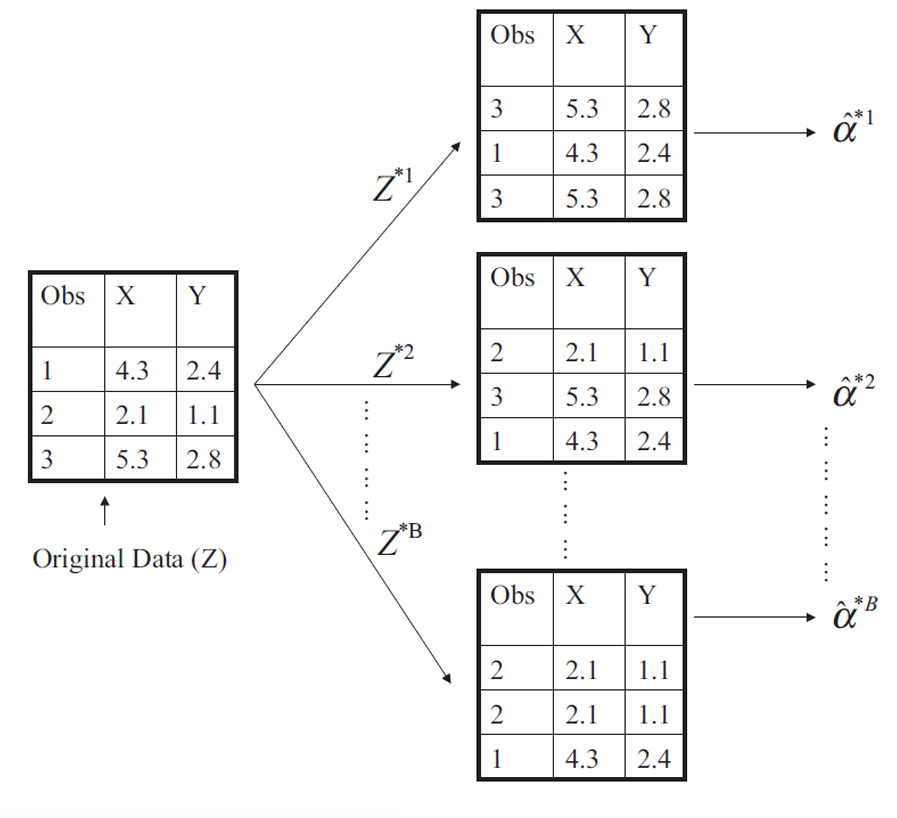
\includegraphics[width=0.5\linewidth]{Images/bootstrapping.png}
    \caption{Bootstrapping}
\end{figure}

This is achieved by repeatedly sampling 
observations from the original data set
Hence, we can estimate the variability of 
an estimator without truly having new 
samples.


The sampling is performed with 
replacement, meaning the observation 
stays in the data set and can be selected (at 
random) again.

In general almost all machine 
learning schemes can be improved by 
building many models on 
bootstrapped data and then 
averaging the response of these 
scheme to a new input.

By training models on multiple bootstrap samples and aggregating
the results (e.g., averaging predictions), bootstrapping reduces the variance of the model.


Computationally this is clearly an 
expensive way to improve 
performance.

\subsubsection{Concept 1} Use the B datasets to
 estimate the uncertainty (e.g.
 standard error) of a method
\subsubsection{Concept 2} Train a separate ML model on each ofthe B datasets and 
average their outcomesto reduce variance

\begin{figure}[H]
    \centering
    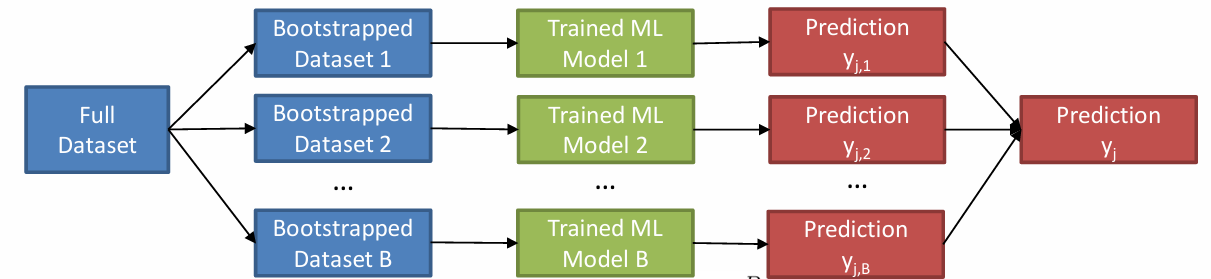
\includegraphics[width=1\linewidth]{Images/bootstrapping-ensemble.png}
    \caption{Ensemble using Bootstrapping}
\end{figure}

\newpage
\section{Regularization}
The goal is to improve:
\begin{description}
    \item[Prediction accuracy] If n is not much larger than p, than least 
    squares results in a high variance. Hence it might not perform well on test 
    observations since it will overfit.

    If n is smaller than p, then there is no 
    unique least squares solution. Adding constraints can help to still find a 
    meaningful solution.
    \item[Model interpretability] Irrelevant predictor variables should be 
    automatically excluded.
\end{description}

\subsection{Subset Selection}
\begin{multicols}{2}
    \subsubsection{Best Subset Selection}
    BSS is a brute force approach with \(2^p\) possible models.

    We first fit a seperate least squares regression to p models having 1 predictor.
    Then we fit seperate regressions to \(\frac{p(p-1)}{2}\) models having 2 predictors and so on.
    Of all the models having \(k\) predictors, only the one with the lowest 
    using \textbf{cross validated} error  is kept: \(M_k\)
    Among these \(p+1\) models the best one is selected.

    Best subset selection is conceptually 
    simple, but it does have a \textbf{major 
    problem, }we need to fit \(2^p\) models.
    It quickly becomes \textbf{computationally 
    infeasible}, and a faster method is needed.

    \begin{figure}[H]
        \centering
        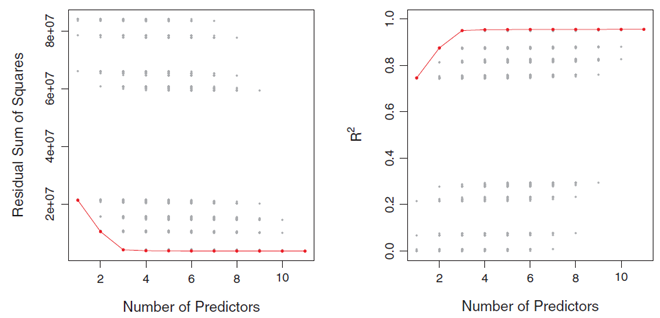
\includegraphics[width=1\linewidth]{Images/best-subset-selection.png}
        \caption{Best Subset Selection}
    \end{figure}

    \subsubsection{Forward Stepwise Selection}
    Once a predictor makes it into the best model, it will stay there.
    The algorithm starts again at the null model but then it will select the model
    with the greatest additional improvement.
    
    Hence this method is a greedy algorithm with only \(p-k\) to be considered.
    At the end the best out of the \(p+1\) 
    models is selected using the cross-validated.

    Forward stepwise selection \textbf{is much more computationally efficient} than best subset selection.
    But it is \textbf{not guaranteed to find the best subset possible}.
    
    \subsubsection{Backward Stepwise Selection}
    This method is almost identical as forward selection but
    unlike forward stepwise selection, 
    it \textbf{requires that a full model can be fit}.
    Therefore \(p\) must be smaller than \(n\) for backward stepwise selection 
\end{multicols}

\subsubsection{Choosing the best model}
In all these approaches, at the end the best model has to be selected.
Since they have different number of predictors, simply \textbf{taking the model with the lowest RSS will not work}.

The proper approach is picking the model with the lowest cross-validated estimated test 
MSE.

\begin{equation*}
    MSE=\frac{RSS}{n}
\end{equation*}

All models under consideration go through a k-fold (k usually 10) crossvalidation procedure to estimate the test 
MSE. The model with the lowest estimated test MSE will be selected.

There is a rule of thumb, as discussed on 
the right, but often one just "eye-balls" and 
picks the lowest possible degree of 
freedom that performs well enough, since 
this will increase the likelihood of 
successful generalization.

\defn{1\(\sigma\)rule-of-thumb}{
    \begin{enumerate}
        \item Calculate standard error for each model size
        \item Pick smallest model within 1\(\sigma\)
        (standard error) of lowest point on curve.
    \end{enumerate}
}

\section{Regularization of Regression Methods (Shrinkage)}
Besides subset selection 
methods, there are two popular 
alternative approaches to \textbf{reduce 
the variance} in the coefficient 
estimates: Ridge regression (Tikhonov 
regularization) and lasso regression.

\subsection{Ridge Regression}

\begin{figure}[H]
    \centering
    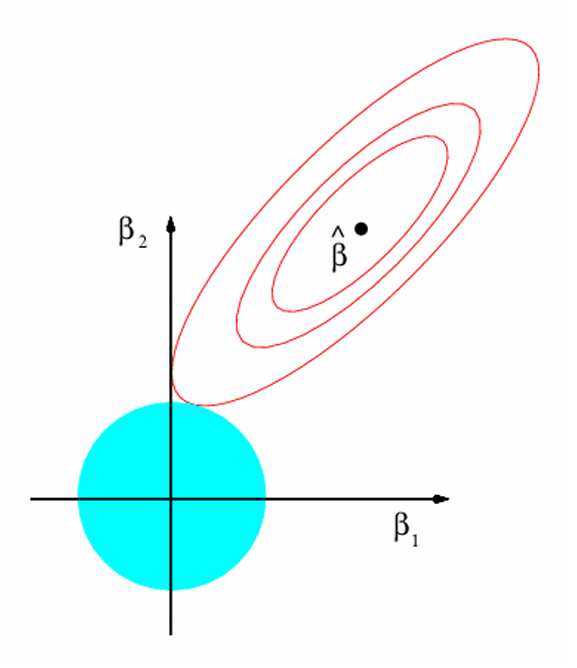
\includegraphics[width=0.35\linewidth]{Images/l2-ellipse.png}
    \caption{L2 ellipse in 2d solution space (\(b_1^2+b_2^2 \leq s\) where s is the budget \(\lambda\))}
\end{figure}

In ridge regression, the idea is that 
coefficients that are closer to zero 
are more desirable.
Therefore the optimization problem, which 
must be solved to find the coefficients of a 
linear model, is extended to favor small 
coefficients over large ones.
The problem is modified so that 
it becomes a trade-off between 
minimizing the RSS and minimizing 
the weighted sum of the squared 
coefficients:
\defn{Ridge Regression}{
    Also called \(L_2\)-Norm (normalization) decreases the coefficients using a wheighted sum:
    \begin{equation}
        min(RSS + \lambda \sum_{j=1}^{p} b_j^2)
    \end{equation}

    It is important that the predictor variables are standardized.
}
Standardization results in the fact, that 
all predictors have a standard deviation of 
one, hence they are all at the same scale.
The weighted sum of the squared coefficients is called the \textbf{shrinkage penalty}.
Since it penalizes the solution for large coefficients it is also called "weight decay".

\begin{figure}[H]
    \centering
    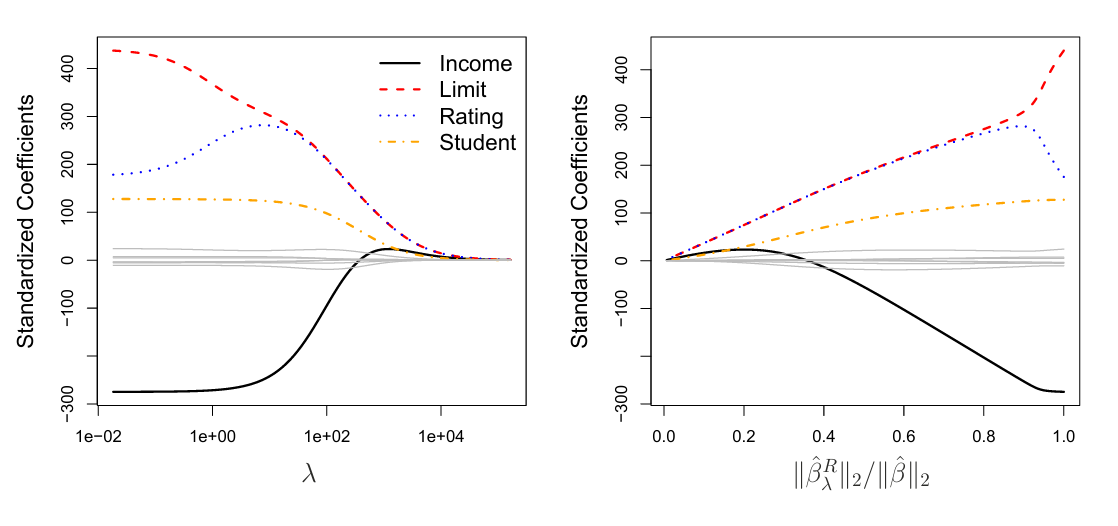
\includegraphics[width=1\linewidth]{Images/l2-norm.png}
    \caption{L2-Normalization}
\end{figure}

\begin{figure}[H]
    \centering
    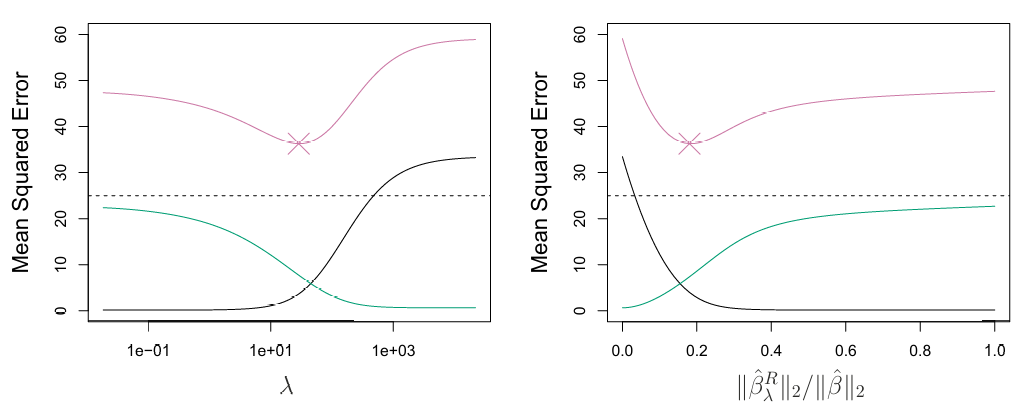
\includegraphics[width=1\linewidth]{Images/l2-bias-variance.png}
    \caption{L2 - Bias Variance: Bias (black), variance (green), MSE (purple)}
\end{figure}

\begin{itemize}
    \item There is an optimal \(\lambda\) (trade-off factor), where the sum of the variance and the \(bias^2\) is 
    minima. It needs to be found separately using \textbf{cross-validation}.
    \item If \(\lambda=0\), then ridge regression is 
    simply the least squares solution, on the other extreme, if \(\lambda\) goes towards infinity, 
    than ridge regression will result in coefficients that are all zero except \(b_0\).
    \item Ridge regression does not remove predictors from the model. This might be no problem for prediction 
    accuracy, but for model interpretation it is nice to have less predictors
\end{itemize}

\subsection{Lasso Regression}
\begin{figure}[H]
    \centering
    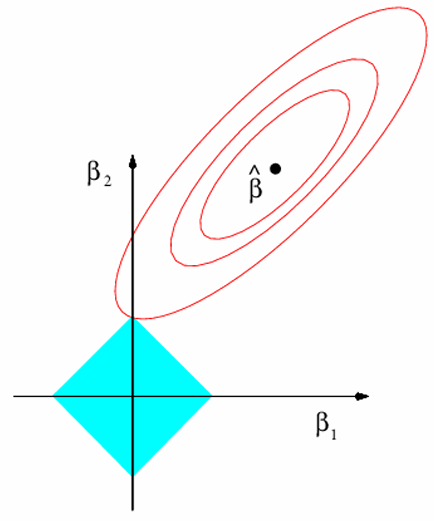
\includegraphics[width=0.35\linewidth]{Images/l1-diamond.png}
    \caption{L1 diamond in 2d solution space (\(|b_1|+|b_2| \leq s\) where s is the budget \(\lambda\))}
\end{figure}


The lasso approach overcomes the limitation of ridge regression,
that no coefficients can be regularized to 0.
The methods are very similar, the only difference is the norm used in the penalty term.

\defn{Lasso}{
    The lasso uses the \(l_1\)-norm (without \(b_0\)).
    Its penalty term also encourages small coefficients and in addition, the \(l_1\) norm will force some 
    coefficients to exactly zero which results in variable selection.

    \begin{equation}
        min(RSS + \lambda \sum_{j=1}^{p} |b_j|)
    \end{equation}
}

\begin{figure}[H]
    \centering
    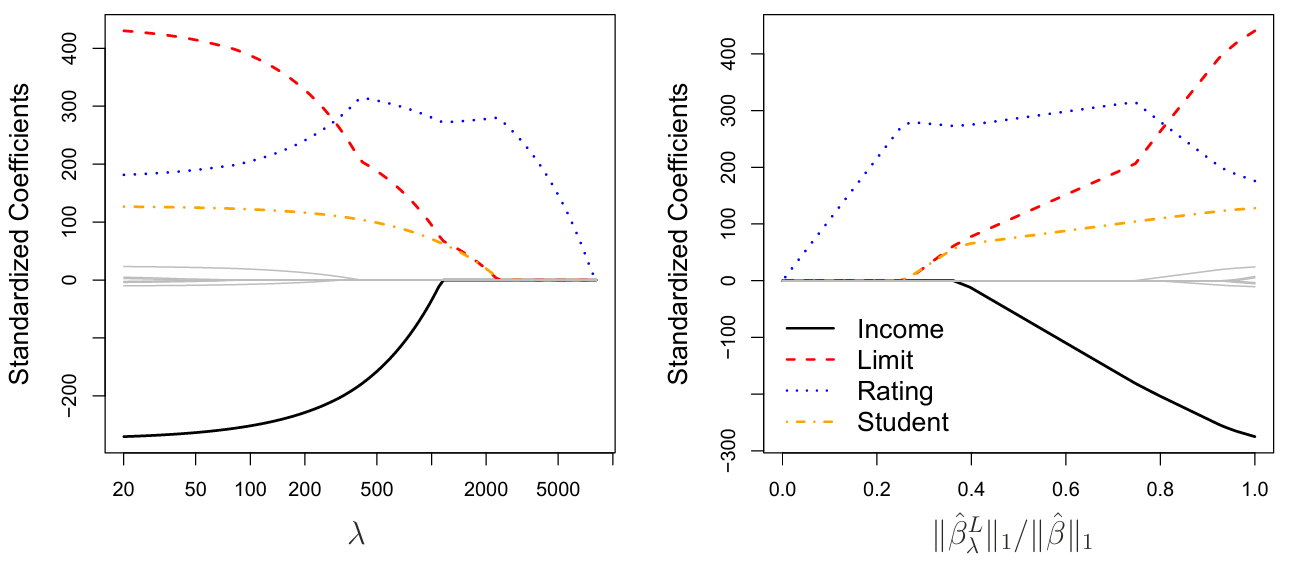
\includegraphics[width=1\linewidth]{Images/l1-norm.png}
    \caption{L1-Normalization}
\end{figure}

\subsection{Comparison}

\begin{figure}[H]
    \centering
    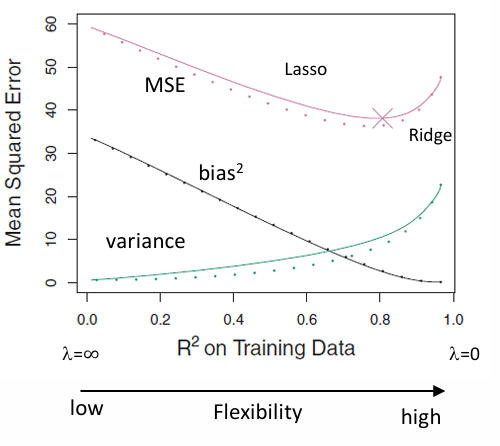
\includegraphics[width=0.5\linewidth]{Images/l1-l2-comparison.png}
    \caption{L1, L2 Comparison}
\end{figure}

\begin{itemize}
    \item One would expect the lasso to perform 
    better when only a small number of 
    predictors have a strong relationship with 
    the response.
    \item One would expect ridge regression to 
    perform better when the response is a 
    function of many predictors all with 
    coefficients of roughly equal size.
    \item Lasso results in models that 
    are simpler to interpret
    \item 
\end{itemize}
As always cross-validation can be used to 
pick the better approach for a particular 
problem at hand.

\subsection{Finding \(\lambda\)}
The pragmatic approach is to choose a grid of \(\lambda\) values and compute the cross validation error.
The \(\lambda\) that results in the lowest crossvalidation error is used to find the coefficients 
sing all the available training data.
\begin{figure}[H]
    \centering
    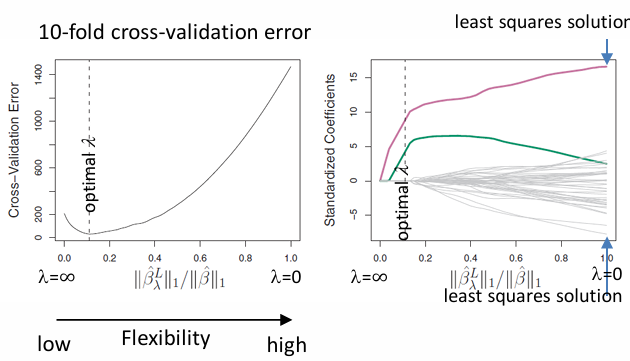
\includegraphics[width=0.75\linewidth]{Images/finding-ld.png}
    \caption{Finding \(\lambda\) with k-Fold=10}
\end{figure}

\newpage
\section{Regularization with Dimensionality Reduction}
Another class of variance reduction schemes first transforms the original predictors
instead of selecting subset or shrinking coefficients.
These approaches are known as dimension reduction methods since 
in the transform domain, we use less than \(p\) variables.

\begin{figure}[H]
    \centering
    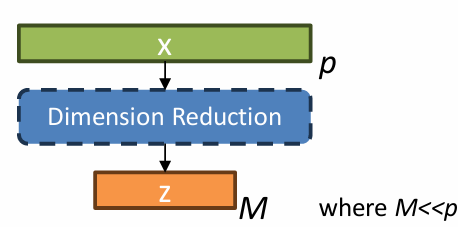
\includegraphics[width=0.5\linewidth]{Images/dim-reduction.png}
    \caption{Dimension Reduction}
\end{figure}

First we need to standardize the predictors:
\begin{equation*}
    \begin{split}
        Z &= \frac{X-\mu}{\sigma} \\
        \tilde{x}_{ij} &= \frac{x_{ij} - \bar{x}_j}{\sqrt{\frac{1}{n}\sum_{i=1}^{n} (x_{ij} - \bar{x}_j)^2}}
    \end{split}
\end{equation*}
Then we reduce the dimensions:
\defn{Basic (Linear) Dimensionality Reduction}{
    Let \(Z_1,\dots,Z_M\) represent \(M<p\) \textbf{linear combinations} of the original predictors.
    The idea is that \(Z\) contain most relevant information:
    \begin{equation}
        Z_m = \sum_{j=1}^{p} \phi_{jm}X_j
    \end{equation}
    \(\phi_{jm}\) are known constants defining the transform it is specific for each \(X_j\)
    and \(Z_M\). The \(Z_M\) are the now new predictors of the model.
}

\begin{figure}[H]
    \centering
    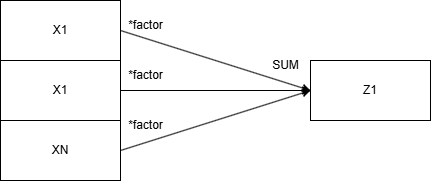
\includegraphics[width=0.5\linewidth]{Images/dim-reduction-schema.png}
    \caption{Dimension Reduction with single \(Z_1\)}
\end{figure}

The term dimension reduction stems from the fact, that in the 
transform domain only \(M+1<p+1\)coefficients need to be estimated.

\subsection{Regression}

\begin{figure}[H]
    \centering
    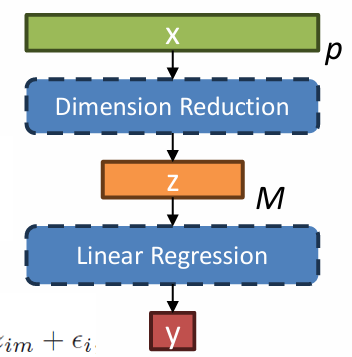
\includegraphics[width=0.25\linewidth]{Images/dim-reduction-regression.png}
    \caption{Dimension Reduction in Regression}
\end{figure}

On lower dimensional data we now can just apply regression as usual,
only the notation changes:

\begin{equation*}
    y_i = \theta_0 + \sum_{m=1}^{M} \theta_m z_{im} + \varepsilon_i
\end{equation*}
Where the coefficients (\(b\)) now are called theta \(\theta_m\).
Now if we plugin the \(Z\) definition into the equation above:
\begin{equation*}
    \begin{split}
        \sum_{m=1}^{M} \theta_m z_{im} &= \sum_{m=1}^{M}  \theta_m \sum_{j=1}^{p} \phi_{jm}x_{ij} \\
        &= \sum_{j=1}^{p} \sum_{m=1}^{M}  \theta_m  \phi_{jm}x_{ij} \\
        &= \sum_{j=1}^{p} b_j x_{ij}
    \end{split}
\end{equation*}
We can see that we still just do linear regression, but we impose restrictions on the \(b_i\).
It is visible that the thetas' \(\theta_m\) are shared among all betas:
\begin{equation*}
    b_j = \sum_{m=1}^{M} = \theta_m \phi_{jm}
\end{equation*}
Constraining the coefficients has the 
potential of biasing the estimate.
However, if \(p\) is large relative to \(n\) 
then selecting a value of \(M<<p\) can 
significantly reduce the variance of 
the fitted coefficients and hence 
more than compensate for the added 
bias (\(MSE=bias2+variance=RSS/n\))

\newpage
\section{Dimensionality Reduction for Regression using Principal Component Analysis (PCA)}

The core idea in PCA is to summarize the information of multiple variables into a new one.
One can think of summarizing the relationship of two variables:

\begin{figure}[H]
    \centering
    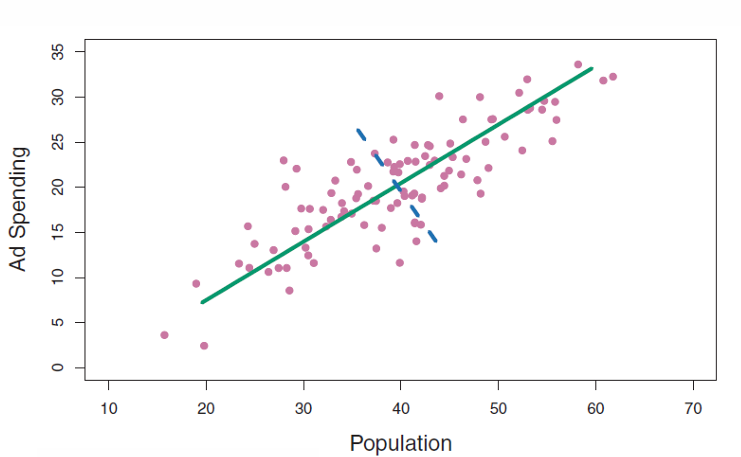
\includegraphics[width=0.75\linewidth]{Images/pca-summarize-relation.png}
    \caption{PCA Line}
\end{figure}

The main goal is to capture as much variance as possible.
The first principal component direction is that along which the observations vary the most.
If the 2D data would be projected onto the first principal component 
then the resulting 1D observations would have the largest possible 
variance of all possible directions to project on.
Projecting a point onto a line simply involves finding the location on the 
line which is the closest to the point, resulting in a perpendicular connecting line.

\begin{figure}[H]
    \centering
    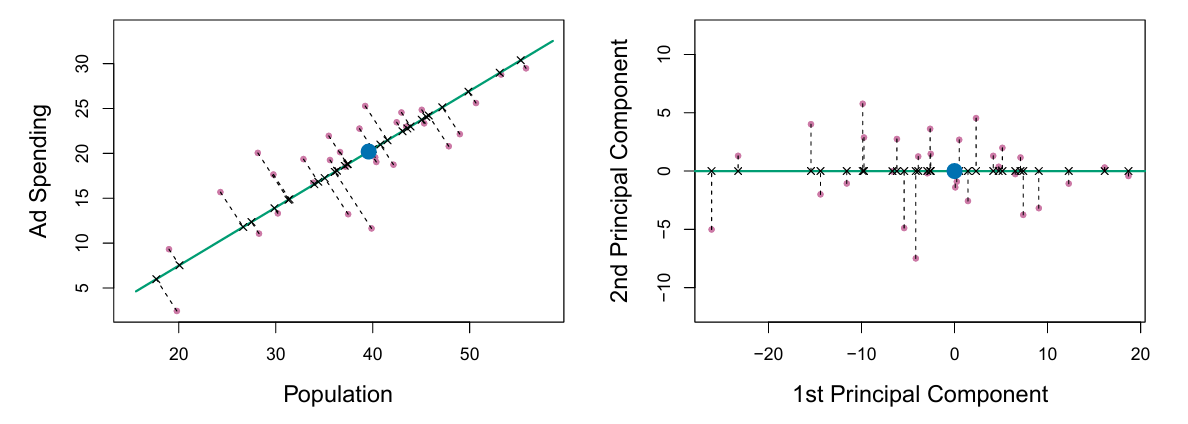
\includegraphics[width=0.75\linewidth]{Images/first-pc.png}
    \caption{Projecting point to the first principal component}
\end{figure}

\defn{PCA}{
    Find a linear transform for principal component for which
    a set of features is a normalized linear combination
    of the features, resulting in the largest variance:
    \begin{equation}
        \begin{split}
            Z_1 &= \phi_{11} X_1 + \phi_{21}X_2+\dots+\phi_{p1}X_p \\
            \text{For which: } Z_1 = &max(var(Z_1))
        \end{split}
    \end{equation}
    \(Z_1\) denotes the first principal component. We choose
    a linear mapping to keep a simple representation.
    One could also choose a non linear transformation (T-SNE).

    With the loading vector of \(Z_1\):
    \begin{equation}
        \phi_1 = (\phi_{11},\dots,\phi_{p1})^T
    \end{equation}
    Each entry \(\phi\) is called loadings of \(Z\).
    The sum of the loadings squared and summed up must equal to 1:
    \begin{equation}
        \sum_{j=1}^{p} \phi_{j1}^2=1
    \end{equation}
    In other words the loadings vector must have norm or length of one.
    Otherwise, the variance can be made arbitrarily large, by selecting
    large loadings.

    Before applying PCA the first step would be to \textbf{normalize the data
    matrix} \(X\). The \textbf{loadings} have a \textbf{geometric meaning}, they show the direction
    of the fit.
}

It is possible to visually see if the predictors are beeing summarized well using PCA:
\begin{figure}[H]
    \centering
    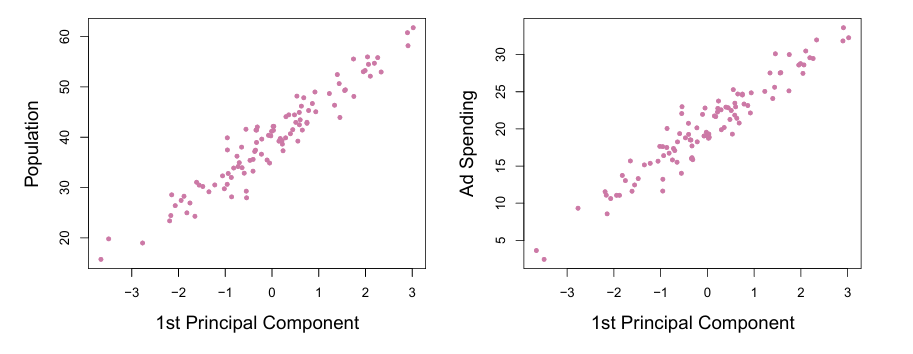
\includegraphics[width=0.75\linewidth]{Images/pca-first-relation.png}
    \caption{First Principal Component}
\end{figure}
If not the data will be more randomly distributed:
\begin{figure}[H]
    \centering
    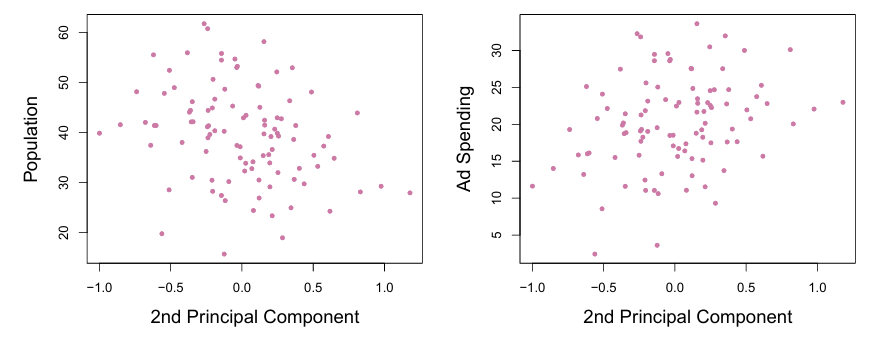
\includegraphics[width=0.75\linewidth]{Images/pca-second-relation.png}
    \caption{Second Principal Component}
\end{figure}
At some time all of the information is more or less captured and adding more
principal components does not work.


\subsection{Further PCs'}
The second principal component is 
also a linear combination of the 
variables having the largest variance 
but with the added constraint, \textbf{that it 
has to be uncorrelated with the first 
principal component}.

This constraint implies that the two 
principal components need to be 
\textbf{orthogonal} (perpendicular) to each 
other.

\subsection{Comparison}
PCA works well if the data is \textbf{highly correlated}.
If it is not, it can well be, that ridge regression works better,
since it can penalize unnecessary predictors or even remove them.
This would be the case if the data is highly independent,
and only a small subset of the predictors are relevant.
This is because PCA cannot remove predictors. Each of the variables
have an effect on the prediction.

PCR biggest drawback is, that there is 
no guarantee that the directions that 
best describe the predictors will also 
be the best directions to describe the 
response.

\subsection{Partial Least Squares}

\begin{figure}[H]
    \centering
    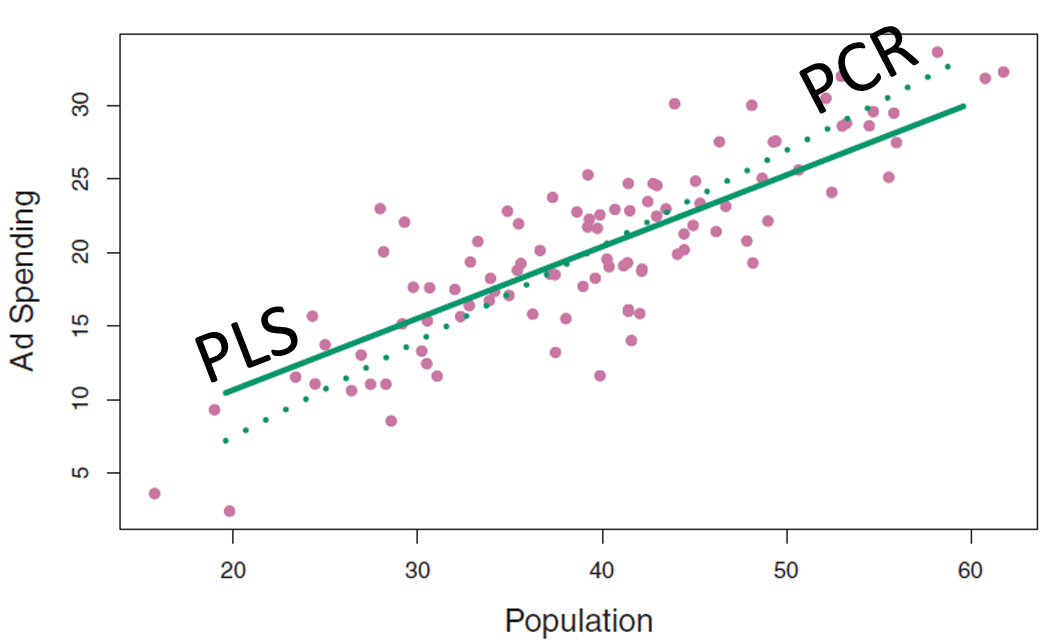
\includegraphics[width=0.75\linewidth]{Images/pcr-pls.png}
    \caption{PLS vs PCR}
\end{figure}
Partial least squares (PLS) is a 
supervised alternative to PCR.
The fundamental idea is to place the highest weight on the predictors that are most strongly 
correlated with the response \(Y\).
PLS often has \textbf{a large variance}, and performs no better than PCR in practice.

\defn{PLS}{
    To find the first PLS direction, the predictors and the response Y 
    are standardized. Now the first direction score \(Z_1\) is 
    computed by setting the \(\phi_{j1}\)'s equal 
    to the \(\beta\)-coefficients from the simple 
    linear regression of \(Y\) onto the \(X_j\)'s.
    These \(\beta\) coefficients are proportional to the 
    \textbf{correlation coefficients} between \(Y\) and the \(X_j\)'s.
}

For further directions we use orthogonalization:
\begin{figure}[H]
    \centering
    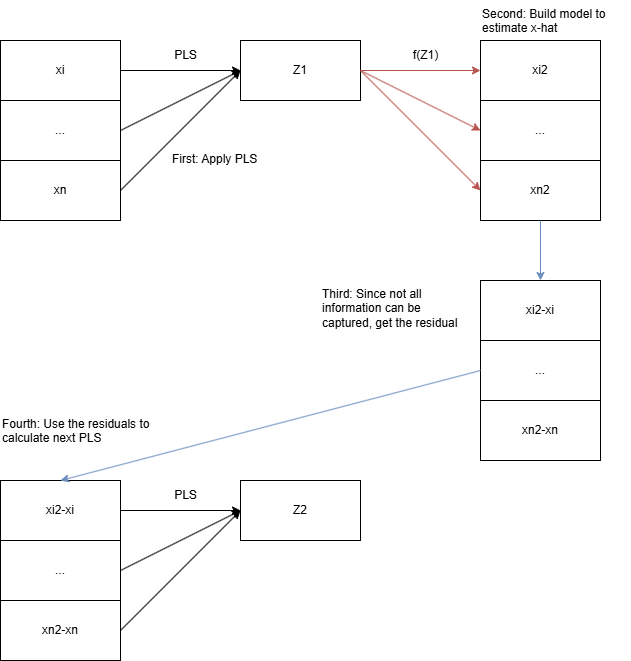
\includegraphics[width=0.5\linewidth]{Images/pls-calculation.png}
    \caption{PLS Calculation}
\end{figure}

\newpage
\section{Considerations in High Dimensions}

\begin{figure}[H]
    \centering
    \includegraphics[width=0.5\linewidth]{Images/high-dim-problems.png}
    \caption{High Variability (High Flexibility/Variance)}
\end{figure}
High dimensionality can have a big impact on model quality.
In comparison to the flexibility a lot of datapoints exist in the upper left figure,
removing some points have a low impact.
Noise will have a lot more strength in high variance situations (upper right figure).
\subsection{Tips for High Dimensionality Problems}
One of the simplest and most effective methods to reduce this effect,
is to apply regularization methods like normalization or dimensionality reduction.
\begin{enumerate}
    \item Shrinkage (also called regularization) plays 
    a key role in high dimensional problem
    \item Appropriate tuning parameter selection is 
    crucial for good predictive performance. Often called "Hyperparameter"
    \item The test MSE tends to increase as the 
    dimensionality of the problem increases. Unless the additional features are truly 
    associated with the response, which we do 
    not know a priori. Hence \textbf{more data is not always better}. The 
    additional \textbf{data needs to be relevant}, i.e., 
    correlated with the response
    \item \(R^2\) is one, this can happen due to \(p=n\) or \(p \approx n\) which will lead to overfitting.
    \textbf{You need to look at the test metrics.} Especially in high dimensions.
    \item Use methods to restrict flexibility: Forward stepwise selection, Ridge, Lasso, PCA
\end{enumerate}

\defn{Curse of Dimensionality}{
    The test MSE tends to increase as the 
    number of predictors increases unless the 
    additional features are truly associated 
    with the response.
    Adding noise features will lead to a 
    deterioration in the fitted model and hence 
    increase the test MSE. Noise features 
    increase the dimensionality of the model, 
    exacerbating the risk of overfitting without 
    improving the test MSE.
    Additionally in high dimensions it is very unikely to that two points are close together.
    This is because there is a high probability that in atleast one dimension, where they
    are far appart.
}

\begin{figure}[H]
    \centering
    \includegraphics[width=0.75\linewidth]{Images/lasso-fails-high-dim.png}
    \caption{Even lasso detiorates in high dimensions of unrelated predictors}
\end{figure}

Multi-collinearty is a major problem 
in high dimensional data.
\textbf{If \(p>n\) then any predictor variable can be 
written as a linear combination of the other 
variables.}
Hence we can never know exactly which 
variables truly are predictive of the 
outcome and we can never identify the 
best coefficients for use in the regression.


\newpage
\section{Tree Based Methods}
Tree-based methods segment the predictor space into a large number of simple regions.
Tree-based schemes are simple and easy to interpret, the performance though is not that great.
Averaging a lot of trees significantly improves the performance at the loss of simplicity and interpretability.

\begin{figure}[H]
    \centering
    \includegraphics[width=0.35\linewidth]{Images/tree-based-methods.png}
    \caption{Tree Terminology}
\end{figure}

\subsection{Building the Tree}
The meaning of Stratification is to divide something into parts or classes.
\begin{enumerate}
    \item (Stratification) Divide predictor space into non-overlapping regions \(R_1,\dots,R_J\).
    This cannot be solved optimally with reasonable computational effort. We use a greedy approach
    (Recursive Binary Splitting).
    \item Define the prediction for every region \(R_j\)
    \begin{itemize}
        \item Inside a region \(R_j\), we make the same prediction (a constant value).
        \item For regression, the best prediction is the 
        sample mean
        \item For classification, we vote.
    \end{itemize}
\end{enumerate}

Algorithm:
\begin{enumerate}
    \item Use recursive binary splitting togrow a large tree.
    \item Apply cost complexity pruning toobtain a sequence of best trees as a function of \(\alpha\).
    \item Use K-fold cross validation to choose \(\alpha\), i.e. for all \(k=1,\dots,K,\) do:
    \begin{enumerate}
        \item Repeat steps 1. and 2. times, using all but the k-th fold as training data.
        \item Calcuate test error on the k-th fold
    \end{enumerate}
    \item Select the best subtree from step 2 with the \(\alpha\) selected in 3.
\end{enumerate}

\subsection{Recursive Binary Splitting (Stratification)}

\defn{Stratification Problem}{
    We want to find boxes \(R_1,\dots,R_J\) that minimizes the RSS:
    \begin{equation}
        min(RSS) \text{ where } RSS = \sum_{j=1}^{J} \sum_{i \in R_j} (y_i - \hat{y_{R_j}})^2
    \end{equation}
    Where \(\hat{y_{R_j}}\) is the average in a corresponding region.
    In classification we use another metric. See sub-section classification.
}

In RBS we only look at the next split and split it optimally.
We always pick the next split which results in the smallest RSS.
This results in many calculation, which are parallelizable.
\begin{figure}[H]
    \centering
    \includegraphics[width=0.5\linewidth]{Images/recursive-binary-splitting.png}
    \caption{Recursive Binary Splitting}
\end{figure}

The same procedure is applied recursively 
to the newly generated regions until a 
stopping criterion is reached.


\begin{figure}[H]
    \centering
    \includegraphics[width=0.75\linewidth]{Images/tree-based-splits.png}
    \caption{Top Left: A partition of two-dimensional feature space that could
    not result from recursive binary splitting. Top Right: The output of recursive
    binary splitting on a two-dimensional example. Bottom Left: A tree corresponding
    to the partition in the top right panel. Bottom Right: A perspective plot of the
    prediction surface corresponding to that tree.}
\end{figure}

\subsection{Cost-Complexity Pruning}
The basic idea is to grow a very large tree and then prune it down to a small one.
\defn{Cost-Complexity Pruning}{
    We use the number of terminal nodes \(|T|\) as a measure of flexibility of a particular tree.
    With this we add a new penalty term:
    \begin{equation}
        \text{minimize: } \sum_{j=1}^{J} \sum_{i \in R_j} (y_i - \hat{y_{R_j}})^2 + \alpha |T|
    \end{equation}

    Now the tuning parameter \(\alpha\) controls the trade-off between RSS reduction and 
    complexity (number of leaves) of the tree. As \(\alpha\) increases the tree becomes simpler.
}
It turns out, as we increase \(\alpha\) from zero, 
branches get pruned from the tree in a 
nested and predictable fashion.

\begin{figure}[H]
    \centering
    \includegraphics[width=0.5\linewidth]{Images/tree-pruning-optimally.png}
    \caption{Next smaller tree (higher \(\alpha\)) is always a subtree of the bigger one}
\end{figure}

\subsection{Classification}

\begin{figure}[H]
    \centering
    \includegraphics[width=0.5\linewidth]{Images/tree-based-classification.png}
    \caption{Tree Based Classification}
\end{figure}

Use winning class \(\hat{k}_m^*\) of region \(m\):
\begin{equation}
    \hat{k}_m^* = argmax(\hat{p}_{mk})
\end{equation}
Where \(\hat{p}_{mk}\) denotes the probabilities for classes \(k\) in region \(m\).

For the probability of the winning class we take:
\begin{equation}
    \hat{p}_m^* = max(\hat{p}_{mk})
\end{equation}
This means our error is:
\begin{equation}
    E_m = 1-max_k(\hat{p}_{mk})
\end{equation}

To grow a classification tree we have to have regions with low \textbf{classification error rate} \(E_m\).
But this does not work well (max operator gets rid of information about losers).
We instead use Gini or Entropy.

\defn{Gini Impurity}{
    Gini Impurity:
    \begin{equation}
        \hat{G}_M = \sum_{k=1}^{K} \hat{p}_{mk} (1-\hat{p}_{mk})
    \end{equation}
    This measures how the probabilities are distributed inside a region.
    If its distributed evenly we get a larger number. Hence it is a measure of node 
    impurity, a low number implies that the node contains predominantly 
    observations from one class, i.e., it is a pure node.
}

\defn{Entropy}{
    \begin{equation}
        \hat{D}_M = -\sum_{k=1}^{K} \hat{p}_{mk} \log \hat{p}_{mk}
    \end{equation}
    If all classes are about equally likely the uncertainty is high and if one 
    class dominates, the uncertainty is low.
}

\begin{itemize}
    \item We build the tree using Gini or Entropy
    \item Pruning can be implemented using Error Rate
    \item Handle categorical values with care since alot of different options are possible,
    if the categories are greater than 2.
\end{itemize}

\subsection{Trees vs Linear Models}
\begin{itemize}
    \item If the relationship is highly non-linear and complex, then decision trees might outperform classical approaches
    \item If the validated performance is comparable, one might prefer the elegant linear regression for its 
    statistical tools or one might prefer a tree based approach for its graphical description
\end{itemize}
\begin{figure}[H]
    \centering
    \includegraphics[width=0.75\linewidth]{Images/tree-vs-linear-models.png}
    \caption{Tree vs Linear Models}
\end{figure}

\subsection{Pro and Cons}
\subsubsection{Pro}
\begin{itemize}
    \item Easy to explain to people
    \item Mirror the human decision-making more closely than e.g. linear regression
    \item Can be displayed graphically
    \item No need for dummy variables when working with qualitative predictors
\end{itemize}
\subsubsection{Cons}
The greatest disadvantage is, that trees generally are \textbf{not as powerful} in 
prediction as some of the other regression and classification approaches.

However, by \textbf{aggregating} many decision trees, using methods like 
bagging and random forest, this disadvantage can be greatly reduced 
so that they are as performant as other methods.

\subsection{Bagging, Random Forests, Out-of-Bag Estimates}

\begin{figure}[H]
    \centering
    \includegraphics[width=0.75\linewidth]{Images/tree-bagging-random-forest.png}
    \caption{Tree with Bagging, Random Forest}
\end{figure}

Decision trees suffer from high variance.
If we for example create a different validation split, the tree may change drastically.
\defn{Bagging}{
    With bagging we create \(B\) independent training datasets using bootstrapping
    and then train \(B\) decision trees. This is called bagging (bootstrap aggregation).
    These trees are grown deep and are not pruned!
    Hence each tree has a high variance but a low bias.
    Averaging these trees reduces the variance.
    In classification we would take majority vote.

    \begin{equation}
        \hat{f}_{bag}(x) = \frac{1}{B} \sum_{b=1}^{B} \hat{f}^{*b}(x)
    \end{equation}
}
While bagging improves prediction accuracy, it comes at the cost of 
interpretability of the model, which used to be one of the advantages of tree-based methods.
When we bag a large number of trees, it is no longer possible to represent the 
resulting statistical learning procedure using a neat single tree and it is no longer 
clear which variables are most important.

\defn{Out-of-Bag Estimates (OOB)}{
    In each bootstraped dataset, take all samples which are not inside the bootstrap-dataset and use these as
    test data to estimate OOB-error on these.
}

\begin{figure}[H]
    \centering
    \includegraphics[width=0.35\linewidth]{Images/random-forest.png}
    \caption{Random Forest}
\end{figure}

\defn{Random Forests}{
    Bagging, but for each split, select a random subset of \(m=\sqrt{p}\) features,
    along which we can split. This reduces correlation among trees!
}

\newpage
\section{Support Vector Machines}
Maximal margin classifiers are used for classifying linearly separable classes.
\textbf{Support vector classifiers} are an extension to maximal margin 
classifiers which also work with linearly not separable classes.
\textbf{Support vector machines} (SVMs) are an extension of support vector classifiers to non-linear boundaries.

\defn{Hyperplane}{
    \begin{equation}
        b_0 + b_1 X_1 + \dots + b_p X_p = 0
    \end{equation}
    From this hyperplane we can define two sides:
    \begin{equation}
        \begin{split}
            b_0 + b_1 X_1 + \dots + b_p X_p &> 0 \\
            b_0 + b_1 X_1 + \dots + b_p X_p &< 0
        \end{split}
    \end{equation}
    We are either on one side of the plane or on the plane itself.
}

Using our data vectors:
\begin{equation*}
    x_1 = \begin{pmatrix}
        x_{11} \\
        \vdots \\
        x_{1p}
    \end{pmatrix}, \dots , x_n
\end{equation*}
We want to find \(b_i\) so that our classes are separated:
\begin{figure}[H]
    \centering
    \includegraphics[width=0.35\linewidth]{Images/max-margin-classifier.png}
    \caption{Binary Classifier}
\end{figure}

Then given a test point \(x^*\), we apply the transform using our \(b_i\) and
check the sign.

We want to remove the if and else statement which occurs from checking the sign.
This can be done by multiplying by \(y_i\):
\begin{equation*}
    y_i (b_0 + b_1 X_1 + \dots + b_p X_p) > 0
\end{equation*}

The margin basically quantifies how close to the hyperplane the closest points are.
The maximal margin hyperplane is the separating hyperplane that has the largest margin to each class of all 
possible separating hyperplanes.

\subsection{Maximal Margin Classifier}
If we select our betas in a special way (beta vector is a unit vector):
\begin{equation*}
    \sum_{j=1}^{p} b_j^2 = 1
\end{equation*}
Then the calculation:
\begin{equation*}
    f(x^*) = b_0 + b_1 x_1^* + \dots + b_p x_p^*
\end{equation*}
Is actually a distance measurement which gives us the perpendicular distance to the line.

\begin{figure}[H]
    \centering
    \includegraphics[width=0.5\linewidth]{Images/max-margin-classifier-2.png}
    \caption{Maximum Margin Classifier}
\end{figure}

\defn{Support Vectors}{
    The points that define the margin are called the support vectors.
    If one has few support vectors they can be analysed and compared.
}

\defn{Maximal Margin Classifiert}{
    In MMC we want to maximize the margin:
    \begin{equation*}
        \text{maximize}_{(b_0,\dots,b_p, \varepsilon_p)} M
    \end{equation*}
    where \(M\) denotes the margin. This must be subjected to:
    \begin{equation*}
        \begin{split}
            \sum_{j=1}^{p} b_j^2 &= 1 \\
            y_i (b_0 + b_1 X_1 + \dots + b_p X_p) &\geq M \quad \forall i = 1, \dots, n
        \end{split}
    \end{equation*}
    The classifier works only for linearly separable data!
    This is a convex optimization problem with one global minimum.
}
\subsection{Support Vector Classifier}

\begin{figure}[H]
    \centering
    \includegraphics[width=0.5\linewidth]{Images/svc.png}
    \caption{Support Vector Classifiert}
\end{figure}

SVC enables non seperable data to be classified.
We want our hyperplane to be able to make errors.
\defn{Support Vector Classifier}{
    In SVC we want to maximize the margin:
    \begin{equation*}
        \text{maximize}_{(b_0,\dots,b_p,\varepsilon_p)} M
    \end{equation*}
    where \(M\) denotes the margin. This must be subjected to:
    \begin{equation*}
        \begin{split}
            \sum_{j=1}^{p} b_j^2 &= 1 \\
            y_i (b_0 + b_1 X_1 + \dots + b_p X_p) &\geq M \quad \forall i = 1, \dots, n
        \end{split}
    \end{equation*}
    as well as:
    \begin{equation}
        y_i (b_0 + b_1 X_1 + \dots + b_p X_p) \geq M(1-\varepsilon_i)
    \end{equation}
    and:
    \begin{equation}
        \varepsilon_i \geq 0, \sum_{i=1}^{n} \varepsilon_i \leq C
    \end{equation}
    \(\varepsilon_i\) are the slack variables it allows an observation to violate the margin.
    \(C\) is budget for violations and is a hyperparameter.

    \begin{equation}
        \begin{split}
            \varepsilon_i = 0 &= \text{all fine}\\  
            0 < \varepsilon_i < 1 &= \text{Within margin} \\
            \varepsilon_i > 1 &= \text{Misclassification}
        \end{split}
    \end{equation}
}
The choice of \(C\) controls the bias variance tradeoff.
If \(C\) is large we increase the margin and thus decrease flexibility
hence lowering variance. We use cross-validation to find \(C\).

This is quite different from many 
other classification methods such as 
the linear discriminant analysis (LDA).
The hyperplane of binary LDA depends on 
all class samples.
Support vector classifiers and logistic 
regression are closely related.

\subsection{Support Vector Machine}
The SVM is an extension of the 
support vector classifier that results 
from enlarging the feature space 
using \textbf{kernels}.

\begin{figure}[H]
    \centering
    \includegraphics[width=0.5\linewidth]{Images/kernel.png}
    \caption{Kernel}
\end{figure}

Kernels are a computationally efficient approach for enlarging the feature space.
It is basically a efficient way to enlarge the feature space without excplicitly
or manually doing so.

One can reformulate and show that the solution
only needs the inner products (dot product) of the observations:
\begin{equation*}
    (x_i, x_{i'}) = \sum_{j=1}^{p} x_{ij} x_{i'j}
\end{equation*}

A linear support vector classifier (the decision function) can be represented with \(n\)
parameters \(\alpha_i\) like this:
\begin{equation*}
    f(x) = b_0 + \sum_{i=1}^{n} \alpha_i (x,x_i)
\end{equation*}

Our line only depends on our support vectors.
\(\alpha_i\) is only non-zero for the sv:
\begin{equation*}
    f(x) = b_0 + \sum_{i \in S} \alpha_i (x,x_i)
\end{equation*}

\begin{figure}[H]
    \centering
    \includegraphics[width=0.75\linewidth]{Images/svm.png}
    \caption{Support Vector Machine}
\end{figure}

We now reformulate our problem to this function:
\defn{SVM Function}{
    \begin{equation*}
        f(x) = b_0 + \sum_{i \in S} \alpha_i K(x,x_i)
    \end{equation*}
    Where \(K\) is a Kernel-Function. Fitting a model
    results in parameters: \(b, \alpha_i\)
}

\defn{Kernel}{
    The kernel trick does a inner product in a high dimensional space.
    Linear Kernel:
    \begin{equation}
        K(x_i, x_{i'}) = \sum_{j=1}^{p} x_{ij} x_{i'j}
    \end{equation}

    Polynomial Kernel of degree \(d\):
    \begin{equation}
        K(x_i, x_{i'}) = (1+\sum_{j=1}^{p} x_{ij} x_{i'j})^d
    \end{equation}

    Gaussian Kernel (RBF,Radial):
    \begin{equation}
        K(x_i, x_{i'}) = exp(-\gamma \sum_{j=1}^{p} (x_{ij} - x_{i'j})^2)
    \end{equation}
    RBF has local behaviour. It takes near points into account and ignore points that are far away.
}
\subsubsection{Multiclass Extension}

\begin{figure}[H]
    \centering
    \includegraphics[width=0.6\linewidth]{Images/one-vs-one.png}
    \caption{One vs One}
\end{figure}
\defn{One vs One}{
    Constructs \( \binom{K}{2} \) binary SVMs'. Which means in total:
    \begin{equation*}
        (K-1) \frac{K}{2} = S
    \end{equation*}
    Of the SVM results, the class that is picked most often is assigned to the test observation.
    This scheme has a problem, when more than one class has the same max number of calls.
    This is resolved e.g. by using a fair coin toss.
}

\defn{One vs All}{
    The class, which results in the larges decision function is assigned to the test observation.
    \begin{equation*}
        K = S
    \end{equation*}
    The magnitude of the function measures the shortest distance from the 
    separating hyperplane in kernel space and 
    the further away from the hyperplane, the more confident we are, that the class 
    decision is the correct one. Furthermore, the function is positive if the 
    sample is classified as belonging to the class k.
}

\begin{figure}[H]
    \centering
    \includegraphics[width=0.6\linewidth]{Images/one-vs-all.png}
    \caption{One vs All}
\end{figure}

\newpage

\section{Unsupervised Learning}
In UL there is no response variable \(Y\), only
predictors \(x_1,\dots ,x_n\). These are measured in
\(n\) observations resulting in the data matrix \(X\)
of dimension \(nxp\). The goal is to gather
inference data using methods like dimensionality reduction
and clustering. The methods require human judgement and have
thus a subjective nature.

\subsection{Principal Component Analysis}
You have your dataset \(X\) up to \(X_p\) with \(n\) rows.
Now you reduce it to include fewer features by incorporating
information into less variables. In PCA regression the idea
was to reduce the dimensions and then to apply a regression model.
This will lead to lower flexibility and thus lower variance.

Without regression we skip the training of a prediction model.
The method stays the same. We try to fit a line to our data
that contains the largest variance.

\begin{figure}[H]
    \centering
    \includegraphics[width=0.6\linewidth]{Images/pve.png}
    \caption{Proportion of Variance Explained}
\end{figure}


\defn{Proportion of Variance Explained (PVE)}{
    Useful for selecting the number of principal
    components to use:
    \begin{equation}
        PVE_m = \frac{\sum_{i=1}^{n} (\sum_{j=1}^{p} \phi_{jm}x_{ij})^2}{\sum_{j=1}^{p}\sum_{i=1}^{n} x_{ij}^2}
    \end{equation}
}

\subsubsection{Scatter-Plot (Biplot)}
PCA is very useful for data visualisation. For example, we
can use PCA to reduce dimension in order to create a scatter plot.
Without PCA the amount of plots would equate to:
\begin{equation}
    \binom{p}{2} = \frac{p(p-1)}{2}
\end{equation}

\begin{figure}[H]
    \centering
    \includegraphics[width=0.5\linewidth]{Images/biplot.png}
    \caption{Biplot}
\end{figure}


\section{Clustering TBD}
\subsection{k-Means Clustering}
\subsection {hierarchical Clustering}

\end{document}